%% The following is a directive for TeXShop to indicate the main file
%%!TEX root = ../../thesis.tex

\chapter{Finite volume electromagnetic modelling on 2D and 3D cylindrical meshes with applications to steel cased wells}
\label{ch:modelling_steel_cased_wells}


\section{Introduction}
\label{sec:intro}

A number of geophysical electromagnetic (EM) problems lend themselves to cylindrical geometries. Airborne EM problems over a 1D earth or borehole-logging applications fall into this category; in these cases cylindrical modelling, which removes a degree of freedom in the azimuthal component, can be advantageous as it reduces the computation load. This is clearly useful when running an inversion where many forward modellings are required, and it  is also valuable to a researcher or a student when exploring and building up an understanding of the behaviour of electromagnetic fields and fluxes in a variety of settings as it reduces feedback time between asking a question and visualizing results (e.g. \cite{Oldenburg2017}).

There are also a range of scenarios where the footprint of the survey is primarily cylindrical, but 2D or 3D variations in the physical property model may be present. For example if we consider a single sounding in an Airborne EM inversion, the primary electric fields are rotational and the magnetic fields are poloidal, but the physical property model may have lateral variations or compact targets. More flexibility is required from the discretization to capture these features. In this case, a 3D cylindrical geometry, which incorporates azimuthal discretization may be advantageous. It allows finer discretization near the source where we have the most sensitivity and the fields are changing rapidly. Far from the source, the discretization is coarser, but it still conforms to the primary behaviour of the EM fields and fluxes and captures the rotational electric fields and poloidal magnetic flux.

In other cases, the most significant physical property variations may conform to a cylindrical geometry, for example in settings where metallic well-casings are present. Understanding the behavior of electromagnetic fields and fluxes in the presence of steel-cased wells is of interest across a range of applications, from characterizing lithologic units with well-logs \citep{Kaufman1990, Kaufman1993, Augustin1989}, to identifying marine hydrocarbon targets \citep{Kong2009, Swidinsky2013, Tietze2015}, to mapping changes in a reservoir induced by hydraulic fracturing or carbon capture and storage \citep{Pardo2013, Borner2015, Weiss2016, Um2015, hoversten2017borehole, Zhang2018}. Carbon steel, a material commonly used for borehole casings, is highly electrically conductive and has a significant magnetic permeability \citep{wuhabashy1994}; it therefore can have a significant influence on electromagnetic signals. The large contrasts in physical properties between the casing and the geologic features of interest, along with the large range of scales that need to be considered to model both the millimeter-thick casing walls while also capturing geologic features, provide interesting challenges and context for electromagnetics in cylindrical geometries. As such, we will use EM simulations of conductive, permeable boreholes as motivation throughout this paper.

In much of the early literature, the casing was viewed as a nuisance which distorts the EM signals of interest. Distortion of surface DC and IP data, primarily in hydrocarbon settings, was examined in \citep{Wait1983, Holladay1984, Johnston1987} and later extended to grounded source EM and IP in \citep{Wait1985, Williams1985, Johnston1992}. Also in hydrocarbon applications, well-logging in the presence of steel cased boreholes is motivation for examining the behavior of electromagnetic fields and fluxes in the vicinity of casing. Initial work focussed on DC resistivity with \citep{Kaufman1990, Schenkel1990, Kaufman1993, Schenkel1994}, and inductive source frequency domain experiments with \citep{Augustin1989}. \citep{Kaufman1990} derives an analytical solution for the electric field at DC in an experiment where an electrode is positioned along the axis of an infinite-length well. The mathematical solutions presented shows how, and under what conditions, horizontal currents leak into the formation outside the well. Moreover, \cite{Kaufman1990} showed, based upon asymptotic analysis, which fields to measure inside the well so that information about the formation resistivity could be obtained. This analysis is extended to include finite-length wells in \cite{Kaufman1993}. \cite{Schenkel1994} show the importance of considering the length of the casing in borehole resistivity measurements, and demonstrate the feasibility of cross-well DC resistivity. They also show that the presence of a steel casing can improve sensitivity to a target adjacent to the well. In frequency domain EM, \citep{Augustin1989} consider a loop-loop experiment, where a large loop is positioned on the surface of the earth and a magnetic field receiver is within the borehole. Magnetic permeability is included in the analysis and a ``casing correction'', effectively a filter due to the casing on inductive-source data, is introduced. This work was built upon for considering cross-well frequency domain EM experiments \citep{Uchida1991, Wilt1996}.

For larger scale geophysical surveys, steel cased wells have been used as ``extended electrodes.'' \cite{Rocroi1985} used a pair of well casings as current electrodes for reservoir characterization in hydrocarbon applications. In near-surface settings \citep{Ramirez1996, Rucker2010, Rucker2012} considered the use of monitoring wells as current and potential electrodes for a DC experiment aimed at imaging nuclear waste beneath a leaking storage tank. Imaging hydraulic fractures has been a motivator for a number of studies at DC or EM, among them \citep{Weiss2016, hoversten2017borehole}. Some of these have suggested the use of casings that include resistive gaps so that currents may be injected in a segment of the well and potentials measured across the other gaps along the well \citep{Nekut1995, Zhang2018}. There has also been a rise in interest in modelling casings for casing integrity applications where the aim of the DC or EM survey is to diagnose if a well is flawed or intact based on data collected on the surface \citep{Wilt2018}.

As computing resources increased, our ability to forward-simulate more complex scenarios has improved, however, the large physical property contrasts and disperate length scales introduced when a steel cased well is included in a model still present a computational challenge. Even the DC problem, which is relatively computationally light, has posed challenges; those are exacerbated when solving the full Maxwell equations in the frequency (FDEM) or time domain (TDEM) and can become crippling for an inversion. For models where the source and borehole are axisymmetric, cylindrical symmetry may be exploited to reduce the dimensionality, and thus number of unknowns, in the problem (e.g. \citep{Pardo2013, Heagy2015}). Highly discretized 3D finite element and finite difference simulations which capture the geometry of the steel cased well have been run at significant computational cost \citep{Commer2015}. To reduce computational load in a 3D simulation, a number of authors have replaced the steel-cased well with a solid borehole, either with the same conductivity as the hollow-cased well (e.g. \citep{Um2015, Puzyrev2017}) or preserving the cross sectional conductance (e.g. \citep{Swidinsky2013}), so that a coarser discretization may be used. \citep{Yang2016} uses a circuit model and introduces circuit components to account for the steel cased well in a 3D DC resistivity experiment. Another approach has been to replace the well with an ``equivalent source'', for example, a collection of representative dipoles, inspired from \citep{cuevas2014}, or with linear charge distributions for a DC problem \citep{Weiss2016}. For the frequency domain electromagnetic problem, a method of moments approach, which replaces the casing with a series of current dipoles, has been taken in \citep{Kohnke2017}.

Capturing the fine-scale features of a conductive, permeable, steel cased well in a 3D electromagnetic simulation is currently in the high-performance computing realm. This means that for a researcher, the tools necessary to investigate the physical behaviour of electromagnetic fields and fluxes, for example, to assess the impact of magnetic permeability or to examine strategies for reducing computational load by making approximations in the forward simulation, are not readily accessible. Our aim in this paper is to bridge that gap.

In this paper, we introduce an approach and associated open-source software implementation for simulating Maxwell’s equations over conductive, permeable models. The simulation domain is discretized in cylindrical coordinates and includes an azimuthal discretization so that non-axisymmetric survey geometries may be considered. Implementations of DC resistivity, frequency domain EM, and time domain EM problems are provided as a part of the SimPEG electromagnetics module \citep{Cockett2015, Heagy2017}. We demonstrate the utility of the implementation for examples that include a steel-cased well in the simulation domain. By using a mesh that conforms to the geometry of the primary EM feature in the model, the steel-cased well, and selecting an appropriate discretization of Maxwell's equations, the number of cells used to discretize the domain can be significantly reduced, as compared to a 3D tensor or OcTree mesh. Our aim in the implementation is to facilitate exploration of the physics, and as such, we have made the fields and fluxes everywhere in the domain readily accessible and provided plotting routines to visualize them. We demonstrate the software with examples at DC, in the frequency domain and in the time domain. Source-code for all examples is provided at https://github.com/simpeg-research/heagy\_2018\_emcyl \citep{Heagy2018}; they are licensed under the permissive MIT license with the hope of reducing the effort necessary by a researcher to compare to or build upon this work.

The paper is organized as follows. In section \ref{sec:numerical_tools}, we introduce the 3D finite volume discretization of Maxwell's equations in cylindrical coordinates and compare a time domain EM simulation to the finite element and finite difference results shown in \citep{Commer2015} as well as a finite volume OcTree simulation described in \citep{Haber2007}. In section \ref{sec:dc_resistivity}, we present two DC resistivity examples. The first follows \citep{Kaufman1990} and shows the behavior of the electric fields, currents, and charges for a long well where an electrode has been positioned along its axis. The second example is inspired from \citep{Kaufman1993} and examines how the currents and charges along the well change with the length of the well. The next example, in section \ref{sec:TDEM}, shows the behavior of currents through time in a ``top-casing'' experiment where one electrode is connected to the well at the surface and a return electrode is positioned some distance away. We examine the currents and the physical phenomena responsible for their distribution through time. Our final example, in section \ref{sec:FDEM} considers a frequency domain experiment inspired by \citep{Augustin1989} and demonstrates the impact of magnetic permeability on the character of the magnetic flux within the vicinity of the borehole and discusses the resulting magnetic field measurements made within a borehole.



\section{Numerical tools}
\label{sec:numerical_tools}

The governing equations under consideration are Maxwell's equations. Under the quasi-static approximation, they are given by:
\begin{equation}
\begin{split}
\nabla \times \vec{e} &= -\frac{\partial \vec{b}}{\partial t} \\
\nabla \times \vec{h} - \vec{j} &= \vec{s}_e
\end{split}
\label{eq:MaxwellTime}
\end{equation}

where $\vec{e}$ is the electric field, $\vec{b}$ is the magnetic flux density, $\vec{h}$ is the magnetic field, $\vec{j}$ is the current density and $\vec{s_e}$ is the source current density. Maxwell's equations can also be formulated in the frequency domain, using the $e^{i \omega t}$ Fourier Transform convention, they are
\begin{equation}
\begin{split}
\nabla \times \vec{E} + i\omega\vec{B} &= 0 \\
\nabla \times \vec{H} - \vec{J} &= \vec{S}_e
\end{split}
\label{eq:MaxwellFreq}
\end{equation}

The fields and fluxes are related through the physical properties: electrical conductivity ($\sigma$, or its inverse, resistivity $\rho$) and magnetic permeability ($\mu$), as described by the constitutive relations
\begin{equation}
\begin{split}
\vec{J} = \sigma \vec{E} \\
\vec{B} = \mu \vec{H}
\end{split}
\label{eq:ConstitutiveRelations}
\end{equation}

At the zero-frequency limit, we also consider the Direct Current Resistivity experiment, described by
\begin{equation}
\begin{split}
\nabla \cdot \vec{j} &= I\left(\delta(\vec{r} - \vec{r}_{s^{+}}) - \delta(\vec{r} - \vec{r}_{s^{-}})\right) \\
\vec{e} &= - \nabla \phi
\end{split}
\label{eq:DCequations}
\end{equation}

where $I$ is the magnitude of the source current density, $\vec{r}_{s^+}$ and $\vec{r}_{s^-}$ are the locations of the current electrodes, and $\phi$ is the scalar electric potential.

Of our numerical tools, we require the ability to simulate large electrical conductivity contrasts, include magnetic permeability, and solve Maxwell’s equations at DC, in frequency and in time in a computationally tractable manner. Finite volume methods are advantageous for modelling large physical property contrasts as they are conservative and the operators ``mimic'' properties of the continuous operators, that is, the edge curl operator is in the null space of the face divergence operator, and the nodal gradient operator is in the null space of the edge curl operator \citep{Hyman1999}. As such, they are common practice for many electromagnetic simulations (e.g. \cite{Horesh2011, Haber2014, Jahandari2014} and references within), and will be our method of choice.

The advantage of cylindrical meshes is that they capture rotational fields and poloidal fluxes characteristic of dipolar EM responses. When the source and physical property model are axisymmetric, cylindrically symmetric meshes, which reduce the dimensionality of the problem, may be employed. A common example of this is when a dipole source is positioned along the axis of a casing in a 1D layered-earth. Under such conditions, simulations which use a fine discretization of the casing can still be solved with modest computational resources. However, for sources offset from the well or for more complex geologic backgrounds,  the problem is fully 3D and accurate modelling must allow for azimuthal variations in the fields and fluxes. Additionally, for applications such as using electromagnetics for diagnosing the integrity of the casing, one may wish to model partial corrosion through the casing, making the steel-cased well an inherently 3D target. To allow such scenarios to be considered, we discretize our computational domain in cylindrical coordinates and include an azimuthal discretization.

\subsection{Discretization}
To represent a set of partial differential equations on the mesh, we use a staggered-grid approach \citep{Yee1966} and discretize fields on edges, fluxes on faces, and physical properties at cell centers, as shown in Figure \ref{fig:CylFiniteVolume}. Scalar potentials can be discretized at cell centers or nodes. Traditionally, a cartesian coordinate system is considered and rectangular cells used for the mesh. As the geometry of steel cased well is cylindrical, we will instead adopt a cylindrical coordinate system. We consider both cylindrically symmetric meshes (Figure \ref{fig:CylFiniteVolume}b) and fully 3D cylindrical meshes, which include a discretization in the azimuthal direction (Figure \ref{fig:CylFiniteVolume}c).


\begin{figure}
    \begin{center}
    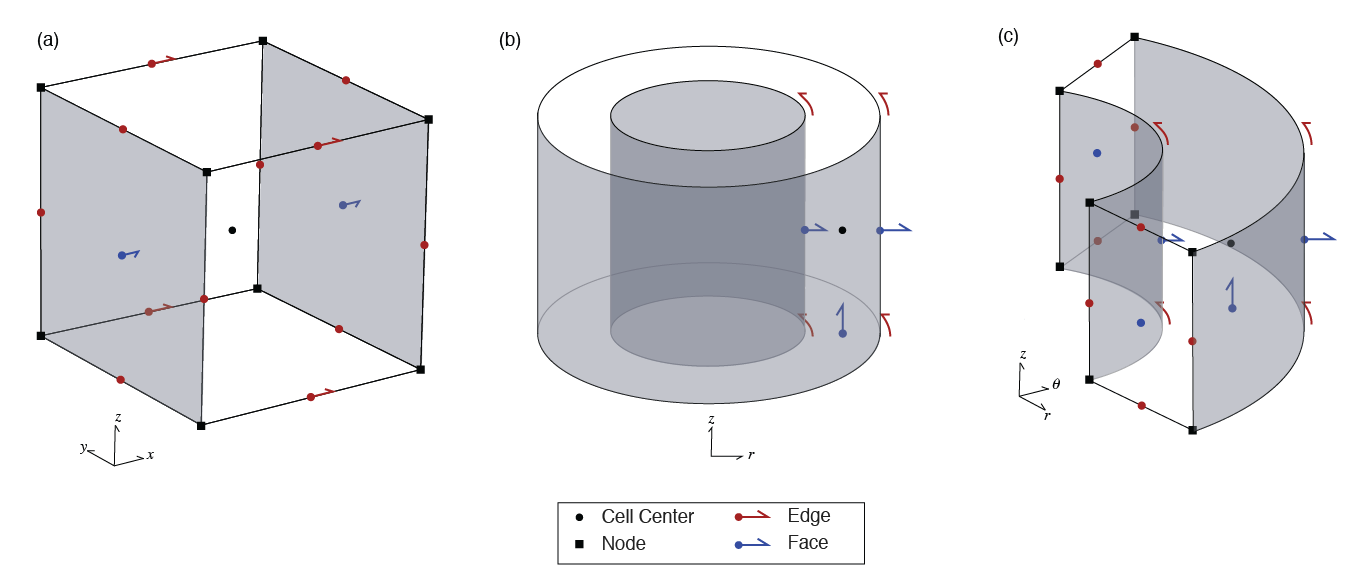
\includegraphics[width=\columnwidth]{figures/casing_software/finiteVolume-02.png}
    \end{center}
\caption{
    Anatomy of a finite volume cell in a (a) cartesian,
    regtangular mesh, (b) cylindrically symmetric mesh, and
    (c) a three dimensional cylindrical mesh.
}
\label{fig:CylFiniteVolume}
\end{figure}


To discretize Maxwell's equations in time (equation \ref{eq:MaxwellTime}) or frequency (\ref{eq:MaxwellFreq}), we invoke the constitutive relations to formulate our system in terms of a single field and a single flux, giving us a system in either the electric field and magnetic flux (E-B formulation), or the magnetic field and the current density (H-J formulation). For example, in the frequency domain, the E-B formulation is
\begin{equation}
    \begin{split}
        \mathbf{C} \mathbf{e} + i\omega\mathbf{b} &= \mathbf{s_m} \\
        \mathbf{C}^\top \mathbf{M}_{\boldsymbol{\mu}^{-1}}^f \mathbf{b} - \mathbf{M}_{\boldsymbol{\sigma}}^e \mathbf{e} &= \mathbf{s_e}
    \end{split}
    \label{eq:DiscreteFDEMEB}
\end{equation}

and the H-J formulation is
\begin{equation}
    \begin{split}
        \mathbf{C}^\top \mathbf{M}_{\boldsymbol{\rho}}^f \mathbf{j} + i\omega\mathbf{M}_{\boldsymbol{\mu}}^e\mathbf{h} &= \mathbf{0} \\
        \mathbf{C} \mathbf{h} - \mathbf{j} &= \mathbf{s_e}
    \end{split}
    \label{eq:DiscreteFDEMHJ}
\end{equation}

where $\mathbf{e}, \mathbf{b}, \mathbf{h}, \mathbf{j}$ are vectors of the discrete EM fields and fluxes; $\mathbf{s_m}$ and $\mathbf{s_e}$ are the discrete magnetic and electric source terms, respectively; $\mathbf{C}$ is the edge curl operator, and the matrices $\mathbf{M}_{\text{prop}}^{e,f}$ are the edge / face inner product matrices. The time-domain equations are discretized in the same manner as is discussed in \citep{Heagy2017}; for time-stepping, a first-order backward Euler approach is used. Although the midpoint method, which is second-order accurate, could be considered, it is susceptible to oscillations in the solution, which reduce the order of accuracy, unless a sufficiently small time-step is used \citep{Haber2004, Haber2014}.

At the zero-frequency limit, each formulation has a complementary discretization for the DC equations, for the E-B formulation the discretization leads to a nodal discretization of the electric potential $\boldsymbol{\phi}$, giving
% \begin{equation}
%     \mathbf{G}^\top \mathbf{M}_{\boldsymbol{\sigma}}^e \mathbf{G} \boldsymbol{\phi} = \mathbf{q}
%     \label{eq:DiscreteDCNodal}
% \end{equation}
\begin{equation}
    \begin{split}
        - \mathbf{G}^\top \mathbf{M}_{\boldsymbol{\sigma}}^e \mathbf{e} &= \mathbf{q} \\
        \mathbf{e} &= -\mathbf{G}\boldsymbol{\phi}
    \end{split}
    \label{eq:DiscreteDCNodal}
\end{equation}

where $\mathbf{G}$ is the nodal gradient operator, and $\mathbf{q}$ is the source term, defined on nodes. Note that the nodal gradient takes the discrete derivative of nodal variables, and thus the output is on edges. The H-J formulation leads naturally to a cell centered discretization of the electric potential
\begin{equation}
    \begin{split}
        \mathbf{V} \mathbf{D}  \mathbf{j} &= \mathbf{q} \\
        \mathbf{M}_{\boldsymbol{\rho}}^f \mathbf{j} &= \mathbf{D}^\top \mathbf{V} \boldsymbol{\phi}
    \end{split}
    \label{eq:DiscreteDCCC}
\end{equation}

Where $\mathbf{D}$ is the face divergence operator, $\mathbf{V}$ is a diagonal matrix of the cell volumes, $\mathbf{q}$ is the source term, which is  defined at cell centers as is $\boldsymbol{\phi}$. Here, the face divergence takes the discrete derivative from faces to cell centers, thus its transpose takes a variable from cell centers to faces. For a tutorial on the finite volume discretization of the DC equations, see \citep{Cockett2016}.

In each of these discrete systems, boundary conditions have been assumed. For the EM simulations, natural boundary conditions are employed; in the E-B formulation, this means $\vec{B}\times\vec{n} = 0\vert_{\partial \Omega}$, and in the H-J formulation, we use $\vec{J}\times\vec{n} = 0\vert{\partial \Omega}$. Within the DC simulations, there is flexibility on the choice of boundary conditions employed; in the simplest scenario, we choose natural boundary conditions. For the nodal discretization, these are Neumann boundary conditions, $\sigma\vec{E} \cdot \vec{n} = 0\vert_{\partial \Omega}$, and for the cell centered discretization, these are Dirichlet boundary conditions $\phi = 0\vert_{\partial \Omega}$.

When employing a cylindrical mesh, the distinction between where the electric and magnetic contributions are discretized in each formulation has important implications. If we consider the cylindrically symmetric mesh (Figure \ref{fig:CylFiniteVolume}b) and a magnetic dipole source positioned along the axis of symmetry (sometimes referred to as the TE mode), we must use the E-B formulation of Maxwell's equation to simulate the resulting toroidal magnetic flux and rotational electric fields. If instead, a vertical current dipole is positioned along the axis of symmetry (also referred to as the TM mode), then the H-J formulation of Maxwell's equations must be used in order to simulate toroidal currents and rotational magnetic fields. The advantage of a fully 3D cylindrical mesh provides additional degrees of freedom, with the discretization in the azimuthal direction, allowing us to simulate more complex responses. However, in order to avoid the need for very fine discretization in the azimuthal direction, we should select the most natural formulation of Maxwell's equations given the source geometry being considered. For a vertical steel cased well and a grounded source, we expect the majority of the currents to flow vertically and radially, thus the more natural discretization to employ is the H-J formulation of Maxwell's equations.

\cite{Haber2014} provides derivations and discussion of the differential operators and inner product matrices; though they are described for a cartesian coordinate system and a rectangular grid, the extension to a three dimensional cylindrical mesh is straightforward. Effectively, a cartesian mesh is wrapped so that the $x$ components become $r$ components, and $y$ components become $\theta$ components, as shown in Figure \ref{fig:cylwrap}.


\begin{figure}
    \begin{center}
    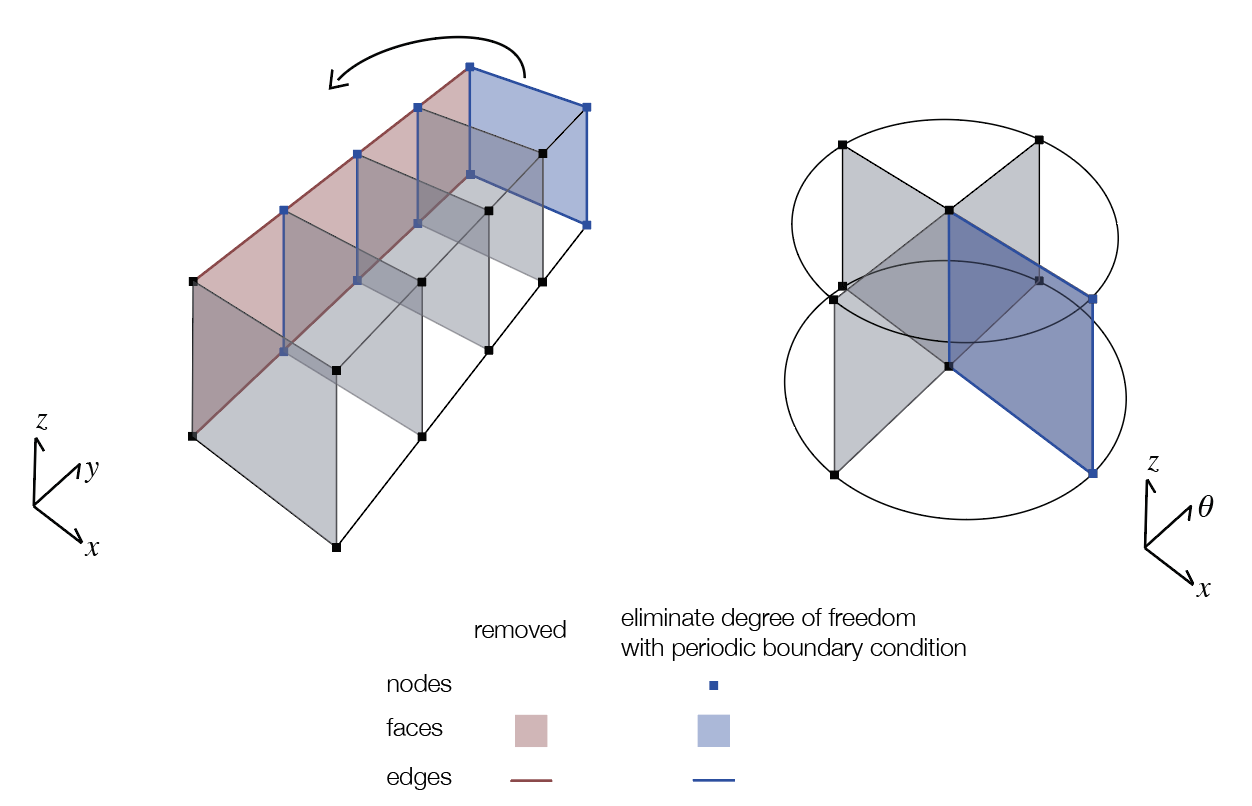
\includegraphics[width=0.9\columnwidth]{figures/cylwrap.png}
    \end{center}
\caption{Construction of a 3D cylindrical mesh from a cartesian mesh.}
\label{fig:cylwrap}
\end{figure}


The additional complications that are introduced are: (1) the periodic boundary condition introduced on boundary faces and edges in the azimuthal direction, (2) the removal of radial faces and azimuthal edges along the axis of symmetry, and (3) the elimination of the degrees of freedom of the nodes and edges at the boundary and as well as the nodes and vertical edges along the axis of symmetry. The implementation of the 3D cylindrical mesh is provided as a part of the \texttt{discretize} package (http://discretize.simpeg.xyz), which is an open-source python package that contains finite volume operators and utilities for a variety of mesh-types. \texttt{discretize} is a part of the larger SimPEG ecosystem \citep{Cockett2015}. All differential operators are tested for second order convergence and for preservation of mimetic properties (as described in \cite{Haber2014}).  The physics engine which solves Maxwell's equations in the time or frequency domain is implemented within SimPEG and described in \cite{Heagy2017}. One of the benefits of SimPEG for forward simulations is that values of the fields and fluxes are readily computed and visualized, which enables researchers to not only simulate data but also examine the physics. This is particularly powerful when combined with the interactive Jupyter environment \citep{Perez2015}.

All of the software used for the following simulations is open source, licensed under the permissive MIT license.  Source code to reproduce the examples shown in this paper are available at: https://github.com/simpegresearch/heagy\_2018\_emcyl.


\subsection{Validation}

Testing for the DC, TDEM, and FDEM implementations includes comparison with analytic solutions for a dipole in a whole-space. These examples are included as supplementary examples in https://github.com/simpegresearch/heagy\_2018\_emcyl. We have also compared the cylindrically symmetric implementation at low frequency with a DC simulations from a Resistor Network solution developed in MATLAB with (Figure 3 in \cite{Yang2016}).

In this paper, we include a comparison with the time-domain electromagnetic simulation shown in Figures 13 and 14 of \cite{Commer2015}. A 200m long well, with a conductivity of $10^{6}$ S/m, outer diameter of 135 mm, and casing thickness of 12 mm is embedded in a 0.0333 S/m background. For the material inside the casing, we use a conductivity equal to that of the background. The conductivity of the air is set to $3 \times 10^{-4}$ S/m and the permeability of the casing is ignored ($\mu = \mu_0$). A 10 m long inline electric dipole source is positioned on the surface, 50m radially from the well. The radial electric field is sampled at 5m, 10m, 100m, 200m and 300m along a line $180^{\circ}$ from the source.

The mesh uses 4 cells radially across the width of the casing, 2.5m vertical discretization, and azimuthal refinement near the source and receivers (along the $\theta=90^\circ$ line), as shown in Figure \ref{fig:commer_mesh}. The mesh has a total of 314 272 cells, and the problem we solve has 948 090 unknowns. For the time discretization, the smallest time-step we use is $10^{-6}$ s; the time-mesh is coarsened at later times. In total, 187 time-steps were used for the simulation, and seven different step-lengths were employed, requiring seven matrix factorizations. To solve the system matrix, the direct solver PARDISO was used \citep{Petra2014, Cosmin2016}. The simulation took 14 minutes to run on a single Intel Xeon X5660 processor (2.80GHz).

Additionally, we compare these results to the 3D UBC finite volume OcTree time-domain code \cite{Haber2014}. The mesh in the UBC simulation included 5 011 924 cells, with the finest cells being equal to the width of the casing; 154 time steps were taken and 10 different step-lengths were used (requiring 10 different matrix factorizations). This simulation took 57 minutes to run on a single Intel Xeon X5660 processor (2.80GHz).



\begin{figure}
    \begin{center}
    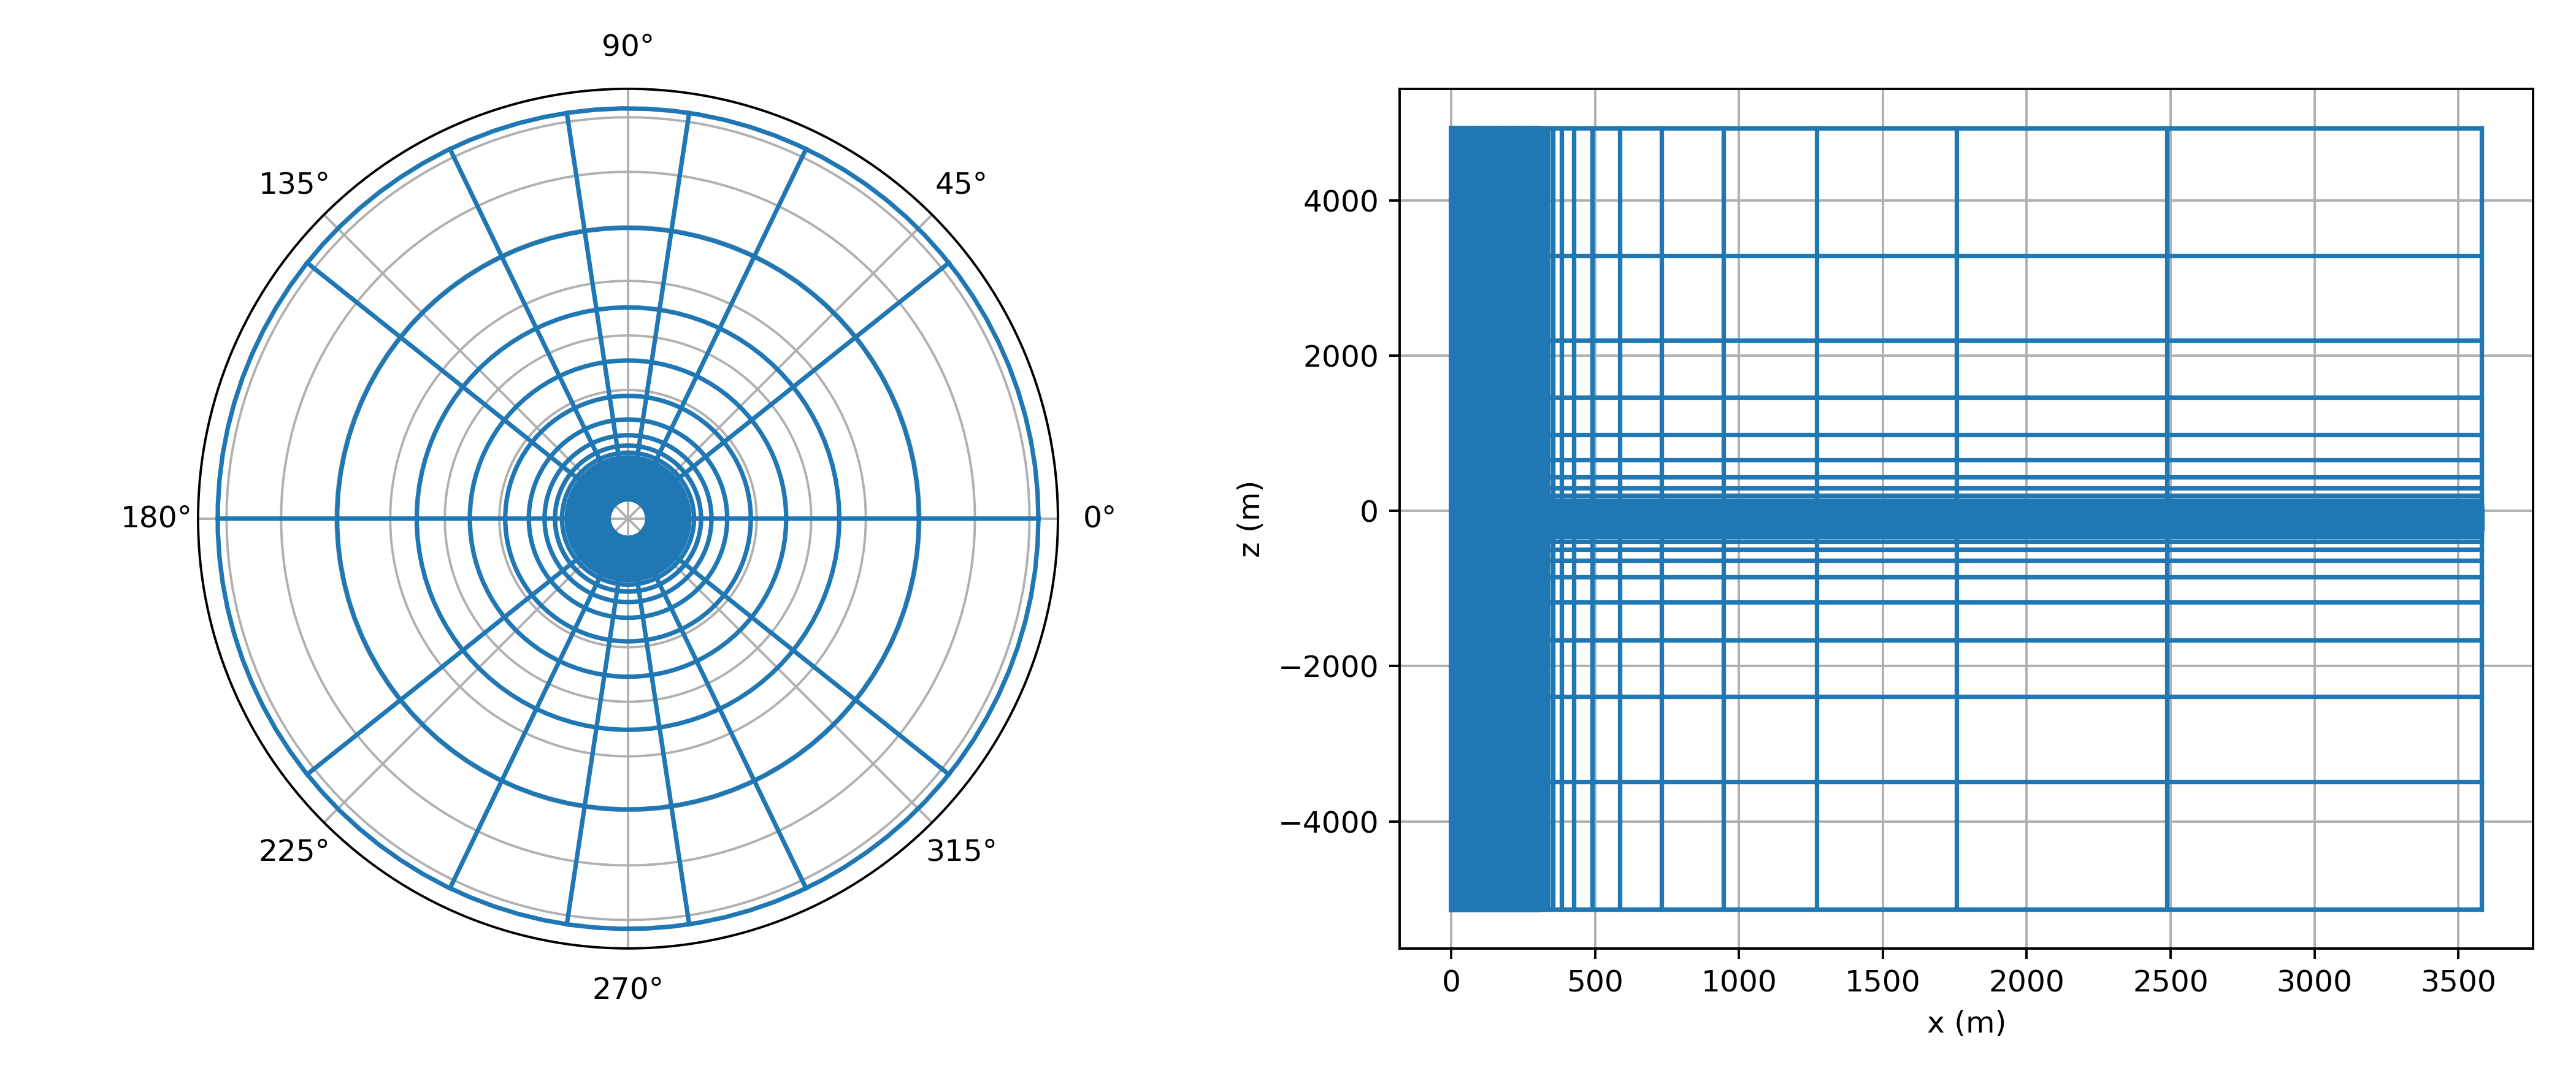
\includegraphics[width=\columnwidth]{figures/commer_mesh.png}
    \end{center}
\caption{Depth slice (left) and cross section (right) through the 3D cylindrical mesh used for the comparison with \cite{Commer2015}. The source and recievers were positioned along the $\theta = 90^\circ$ line.}
\label{fig:commer_mesh}
\end{figure}



In Figure \ref{fig:commer_results}, we show the absolute value of the radial electric field sampled at fives stations; each of the different line colors is associated with a different location, and offsets are with respect to the location of the well. The 3D cylindrical simulation (SimPEG) is plotted with a solid line and overlaps with the UBC solution (dash-dot line) for all times shown. The finite element (FE) solution from \cite{Commer2015} is shown with the dashed lines, and the finite difference (FD) solution is plotted with dotted lines. The 3D cylindrical (SimPEG) and UBC solutions are overall in good agreement with the solutions from \cite{Commer2015}. There is a difference in amplitude and position of the zero-crossing (the v-shape visible in the blue and orange curves) between the Commer solutions and the SimPEG / UBC solutions at the shortest two offsets in the early times. At such short offsets from a highly conductive target, details of the simulation such as averaging, interpolation and discretization become significant; this likely accounts for the discrepancies but a detailed code-comparison is beyond the scope of this paper. Our aim with this comparison is to provide evidence that our numerical simulation is performing as expected, and we deem that our overall agreement with Commer’s and UBC’s results is confirmation of this.


\begin{figure}[htb]
    \begin{center}
    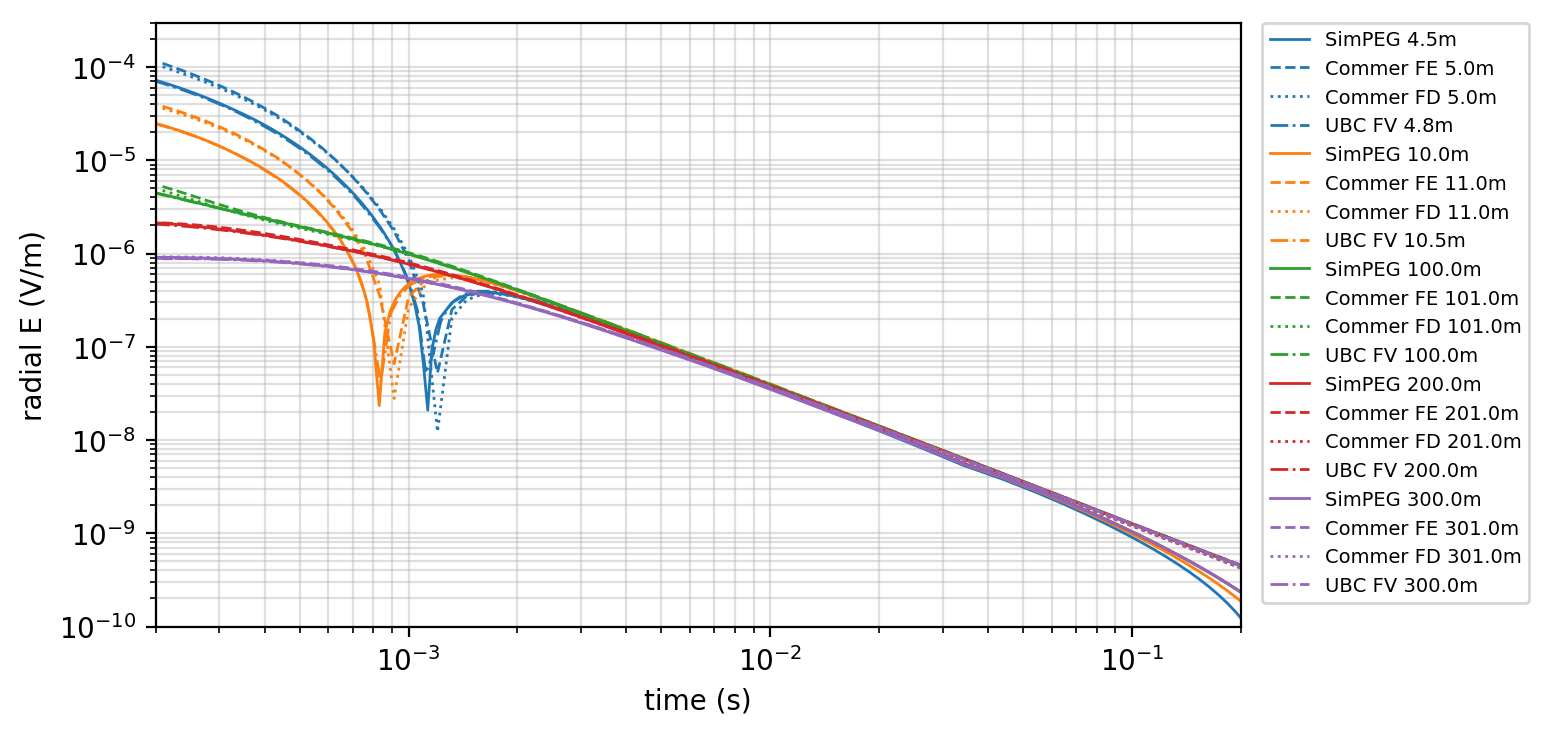
\includegraphics[width=\columnwidth]{figures/commer_results.png}
    \end{center}
\caption{Time domain EM response comparison with \citep{Commer2015}. Each of the different line colors is associated with a different location; offsets are with respect to the location of the well.}
\label{fig:commer_results}
\end{figure}





\section{Numerical Examples}
\label{sec:numerical_results}

We demonstrate the implementation through examples using the DC, time-domain EM and frequency domain EM codes. To focus discussion, each of the examples explores an aspect of the physical behavior of electromagnetic fields and fluxes in the presence of a steel-cased well. Though the codes are general, we choose to focus on this application because it is numerically challenging, the physics is complicated and the technique has practical applications that are currently being pursued.
\subsection{DC Resistivity}
\label{sec:dc_resistivity}

In his two seminal papers on the topic, Kaufman uses transmission line theory to draw conclusions about the behaviour of the electric field when an electrode is positioned inside of an infinite casing. In this first example, we will revisit some of the physical insights discussed in \citep{Kaufman1990, Kaufman1993} that followed from an analytical derivation and compare those to our numerical results. In the second example, we look at the distribution of current and charges as the length of the well is varied and compare those to the analytical results discussed in \citep{Kaufman1993}.

\subsubsection{Example 1: Electric fields and currents in a long well}

We start by considering a 1km long well ($10^6$ S/m) in a whole space ($10^{-2}$ S/m), with the conductivity of the material inside the borehole equal to that of the whole space.  For modelling, we will use a cylindrically symmetric mesh. The positive electrode is positioned on the borehole axis in the mid-point of a 1km long well;  a distant return electrode is positioned 1km away at the same depth.

Kaufman discusses the behavior of the electric field by dividing the response into three zones: a near zone, an intermediate zone and a far zone \citep{Kaufman1990, Kaufman1993}. In the near zone, the electric field has both radial and vertical components, negative charges are present on the inside of the casing, and positive charges are present on the outside of the casing. The near zone is quite localized and typically, its vertical extent is no more than $\sim 10$ borehole radii away from the electrode. To examine these features in our numerical simulation, we have plotted in Figure \ref{fig:kaufman_zones}: (a)  the total charge, (b) secondary charges, (c) electric field, and (d) current density in a portion of the model near the source. The behaviours expected by Kaufman are consistent with our numerical results.

Within the near-zone, the total charge is dominated by the large positive charge at the current electrode location and negative charges that exist along the casing wall where current is moving from a resistive region inside the borehole into a conductor. The extent of the negative charges along the inner casing wall is more evident when we look at the secondary charge, which is obtained by subtracting the charge that would be observed in a uniform half-space from the total charge (Figure \ref{fig:kaufman_zones}b). Inside the casing, we can see the transition from near-zone behavior to intermediate zone behavior approximately 0.5 m above and below the source; that is equal to 10 borehole radii from the source location, which agrees with Kaufman's conclusion.

In the intermediate zone, Kaufman discusses a number of interesting aspects with respect to  the behavior of the electric fields and currents which we can compare with the observed behavior in Figure \ref{fig:kaufman_zones}. Among them, he shows that the electric field within the borehole and casing is directed along the vertical axis; as a result no charges accumulate on the inner casing wall. Charges do, however, accumulate on the outer surface of the casing; these  generate radially-directed electric fields and currents, often referred to as “leakage currents”, within the formation. At each depth slice through the casing and borehole, the electric field is uniform, however, due to the high conductivity of the casing, most of the current flows within the casing.  The vertical extent of the intermediate zone depends on the resistivity contrast between the casing and the surrounding formation and extends beyond several hundred meters before transitioning to the far zone, where the influence of the casing disappears \citep{Kaufman1990}.


\begin{figure}
    \begin{center}
    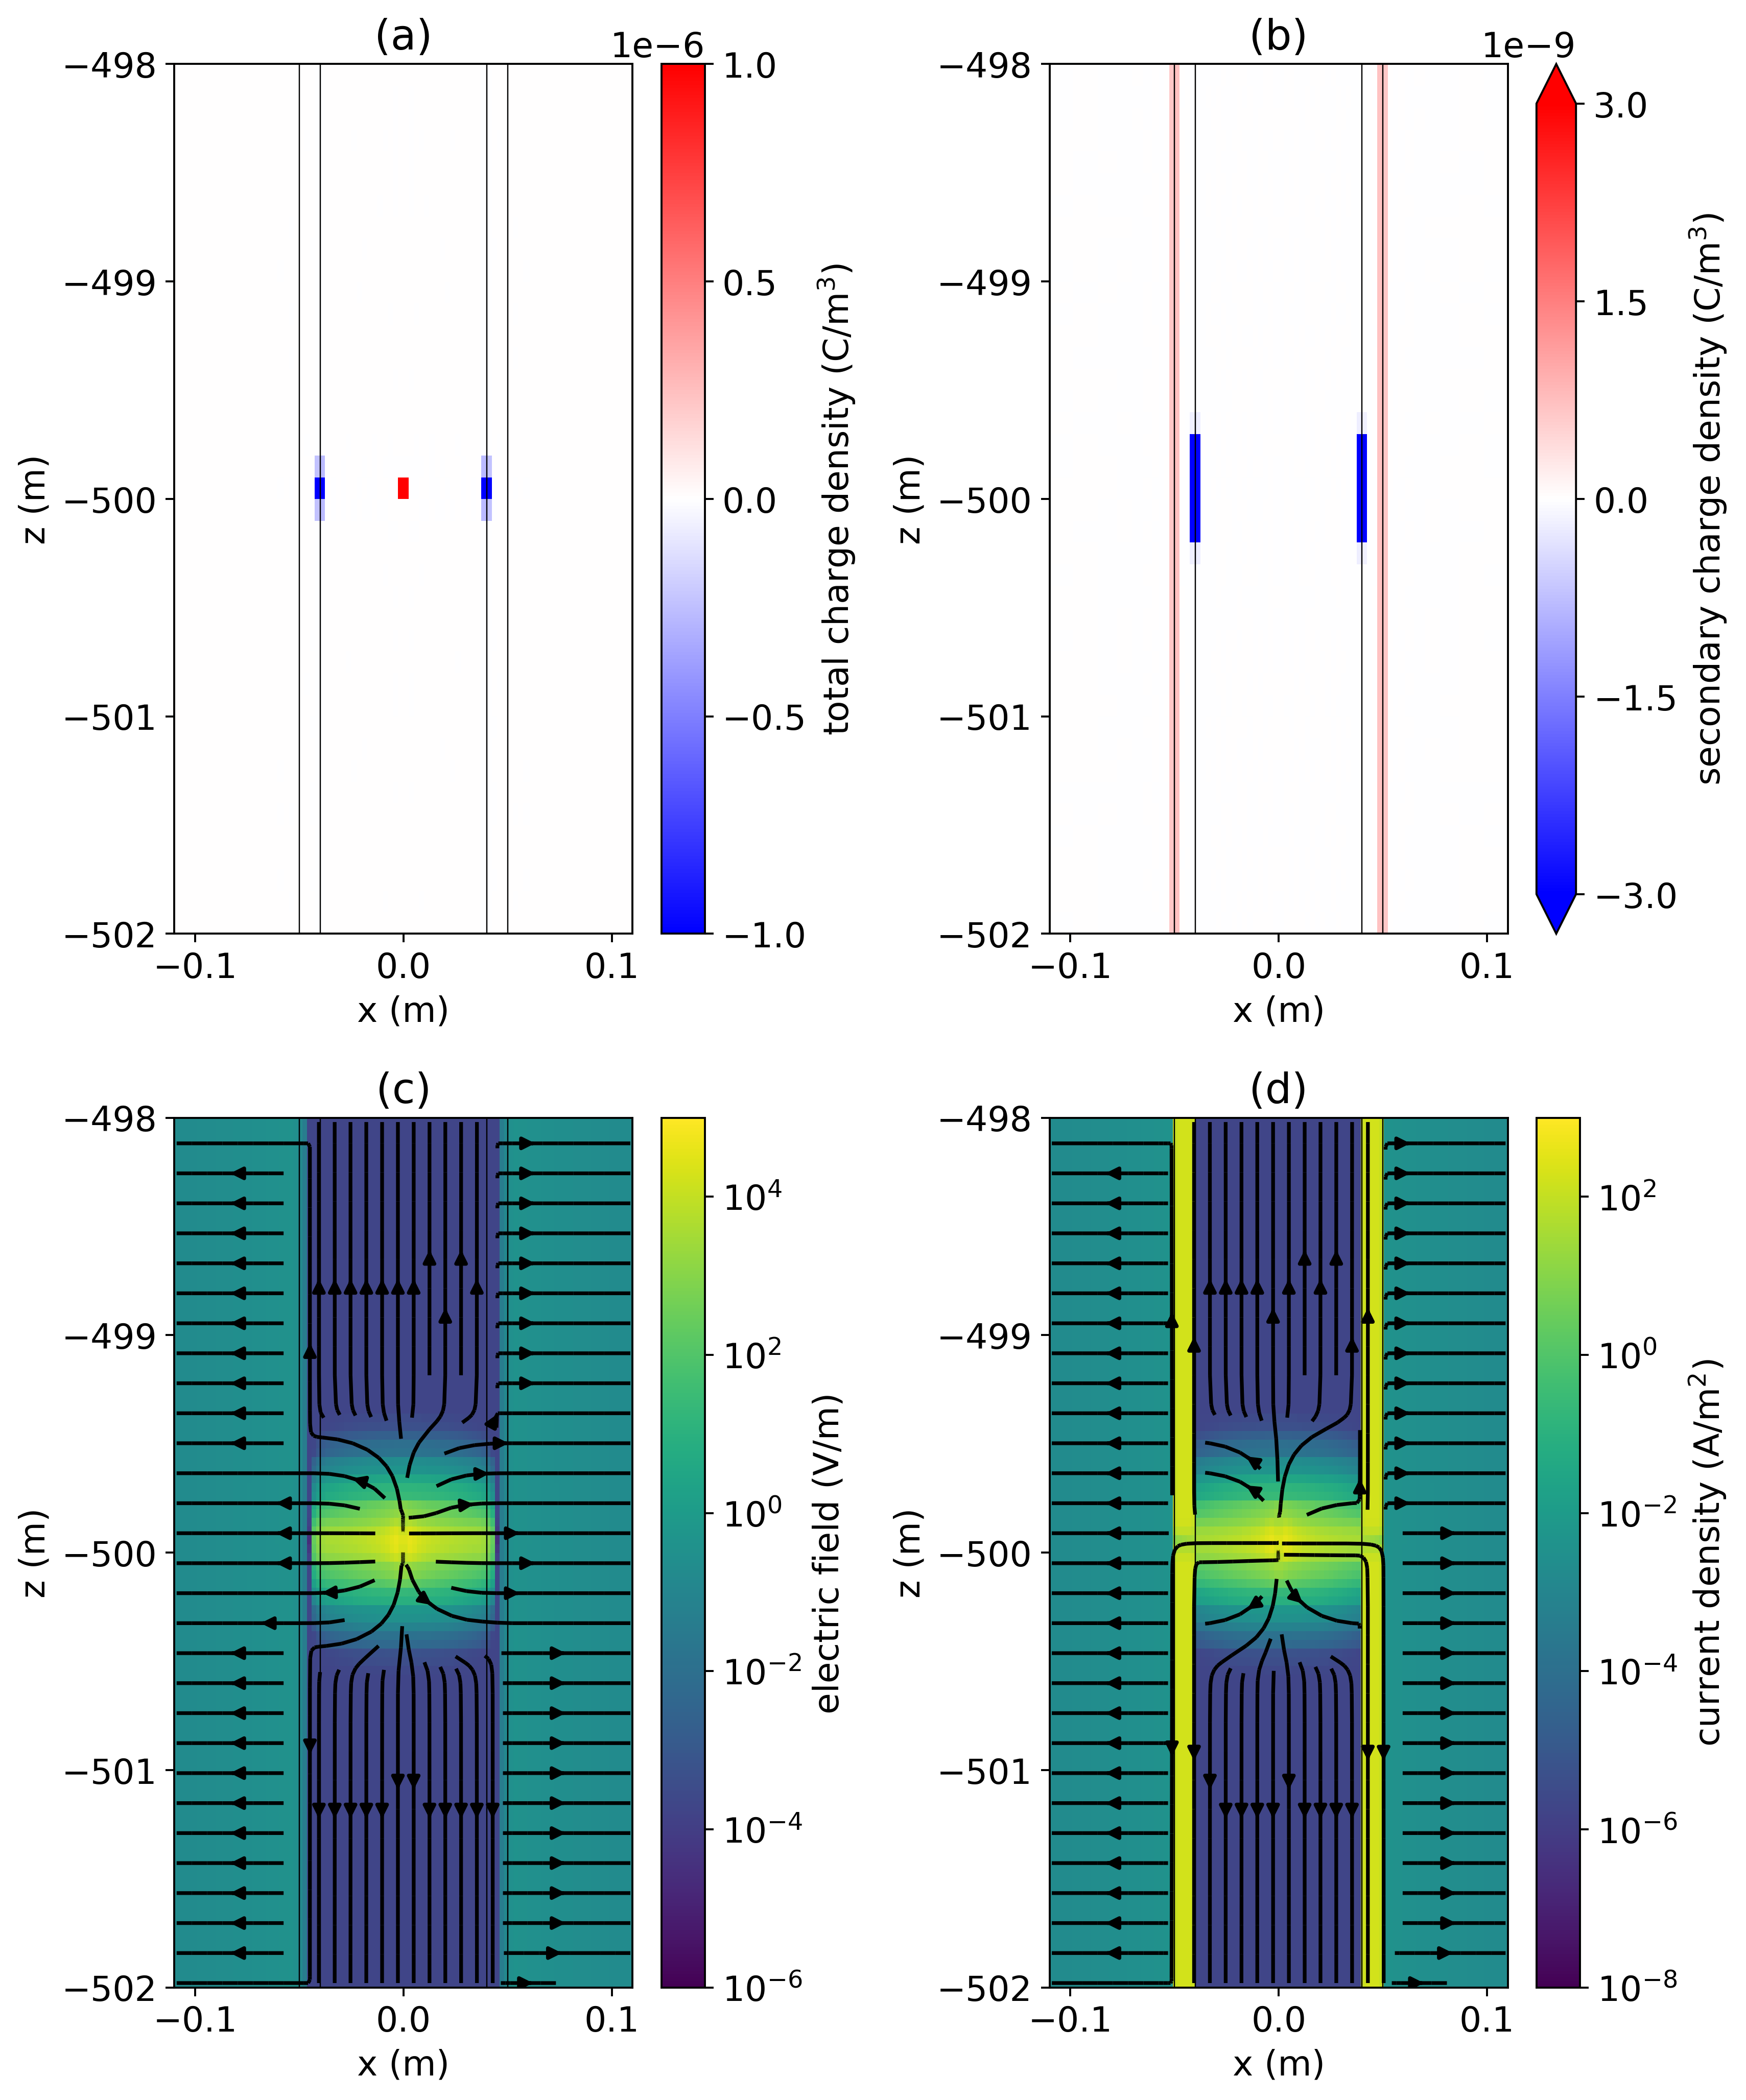
\includegraphics[width=0.7\columnwidth]{figures/casing_software/kaufman_zones.png}
    \end{center}
\caption{(a) Total charge density, (b) secondary charge density, (c) electric field, and (d) current density in a section of the pipe near the source at z=-500m.}
\label{fig:kaufman_zones}
\end{figure}



The radially directed fields from the casing, and the length of the intermediate zone, have practical implications in the context of well-logging because they delineate the region in which measurements can be made to acquire information about the formation resistivity outside the well. Within the intermediate zone, fields behave like those due to a transmission line \citep{Kaufman1990}, and multiple authors have adopted modelling strategies that approximate the well and surrounding medium as a transmission line \citep{Kong2009, Aldridge2015}. We will extend this analysis in the next example and discuss how the length of the well impacts the behavior of the charges, fields, and fluxes.
\subsubsection{Example 2: Finite Length Wells}
\label{sec:finite_length_well}

In \citep{Kaufman1993}, the transmission-line analysis was extended to consider finite-length wells. Inspired by the interest in using the casing as an ``extended electrode'' for delivering current to depth (e.g. \citep{Schenkel1994, Um2015, Weiss2016, hoversten2017borehole}), here we consider a 3D DC resistivity experiment where one electrode is connected to the top of the well. We will examine the current and charge distribution for wells ranging in length from 250m to 4000m and compare those to the observations in \citep{Kaufman1993}. The conductivity of the well is selected to be $10^6$ S/m. A uniform background conductivity of $10^{-2}$ S/m is used and the return electrode is positioned 8000m from the well; this is sufficiently far from the well that we do not need to examine the impact of the return electrode location in this example. A 3D cylindrical mesh was used for the simulation.

\citep{Kaufman1993} derives a solution for the current within a finite length well and discusses two end-member cases: a short well and a long well. ``Short'' versus ``long'' are defined on the product of $\alpha L_c$, where $L_c$ is the length of the casing and $\alpha = 1/\sqrt{S T}$, where $S$ is the cross-sectional conductance of the casing and has units of S$\cdot$m ($S = \sigma_c 2\pi a \Delta a$, for a casing with radius $a$ and thickness $\Delta a$), and $T$ is the transverse resistance. The transverse resistance  is approximately equal to the resistivity of the surrounding formation (for more discussion on where this approximation breaks down, see \cite{Schenkel1994}). For short wells, $\alpha L_c \ll 1$, the current decreases linearly with distance, whereas for long wells, where $\alpha L_c \gg 1$, the current decays exponentially with distance from the source, with the rate of decay being controlled by the parameter $\alpha$. In Figure \ref{fig:kaufman_finite_well} (a), we show current in the well for 5 different borehole lengths. The x-axis is the distance from the source normalized by the length of the well. We also show the two end-member solutions (equations 45 and 53) from \cite{Kaufman1993}. There is significant overlap between the 250m numerical solution and the short well approximation. As the length of the well increases, exponential decay of the currents becomes evident. Since $\alpha$ is quite small, for this example $\alpha = 2 \times 10^{-3} m^{-1}$, the borehole must be very long to reach the other end member which corresponds to the exponentially decaying solution.

In Figure \ref{fig:kaufman_finite_well} (b), we have plotted the charges along the length of the well. In the short-well regime, the borehole is approximately an equipotential surface and the charges are uniformly distributed; in the long well the charges decay with depth. What was surprising to us was the noticeable increase in charge accumulation that occurs near the bottom of the well. This is especially evident for the short well. Initially, we were suspicious and thought this might be due to problems with our numerical simulation; there was no obvious physical explanation that we were aware of. However, investigation into the literature revealed that the increase in charge density at the ends of a cylinder is a real physical effect, but an exact theoretical solution does still not appear to exist \citep{Griffiths1997} (see Figure 4, in particular).

The results shown in Figure \ref{fig:kaufman_finite_well} have implications when testing approaches for reducing computational load by approximating a well with a solid tube or prism, as in \cite{Um2015}, or replacing the well with a distribution of charges, as in \cite{Weiss2016}. For a short well, the behaviour of the currents is independent of conductivity, so, as long as the borehole is approximated by a sufficiently conductive target, the behaviour of the fields and fluxes will be representative of the fine-scale model. However, as the length of the well increases, the cross-sectional conductance of the well, becomes relevant as it controls the rate of decay of the currents in the well and thus the rate that currents leak into the formation. A similar result holds when a line of charges is used to approximate the well as a DC source; a uniform charge is suitable for a sufficiently short or sufficiently conductive well, whereas a distribution of charge which decays exponentially with depth needs to be considered for longer wells. Thus, when attempting to replace a fine-scale model of a well with a coarse-scale model, either with a conductivity structure or by some form of ``equivalent source'', validations should be performed on models that have the same length-scale as the experiment to ensure that both behaviors are being accurately modeled.


\begin{figure}[htb]
    \begin{center}
    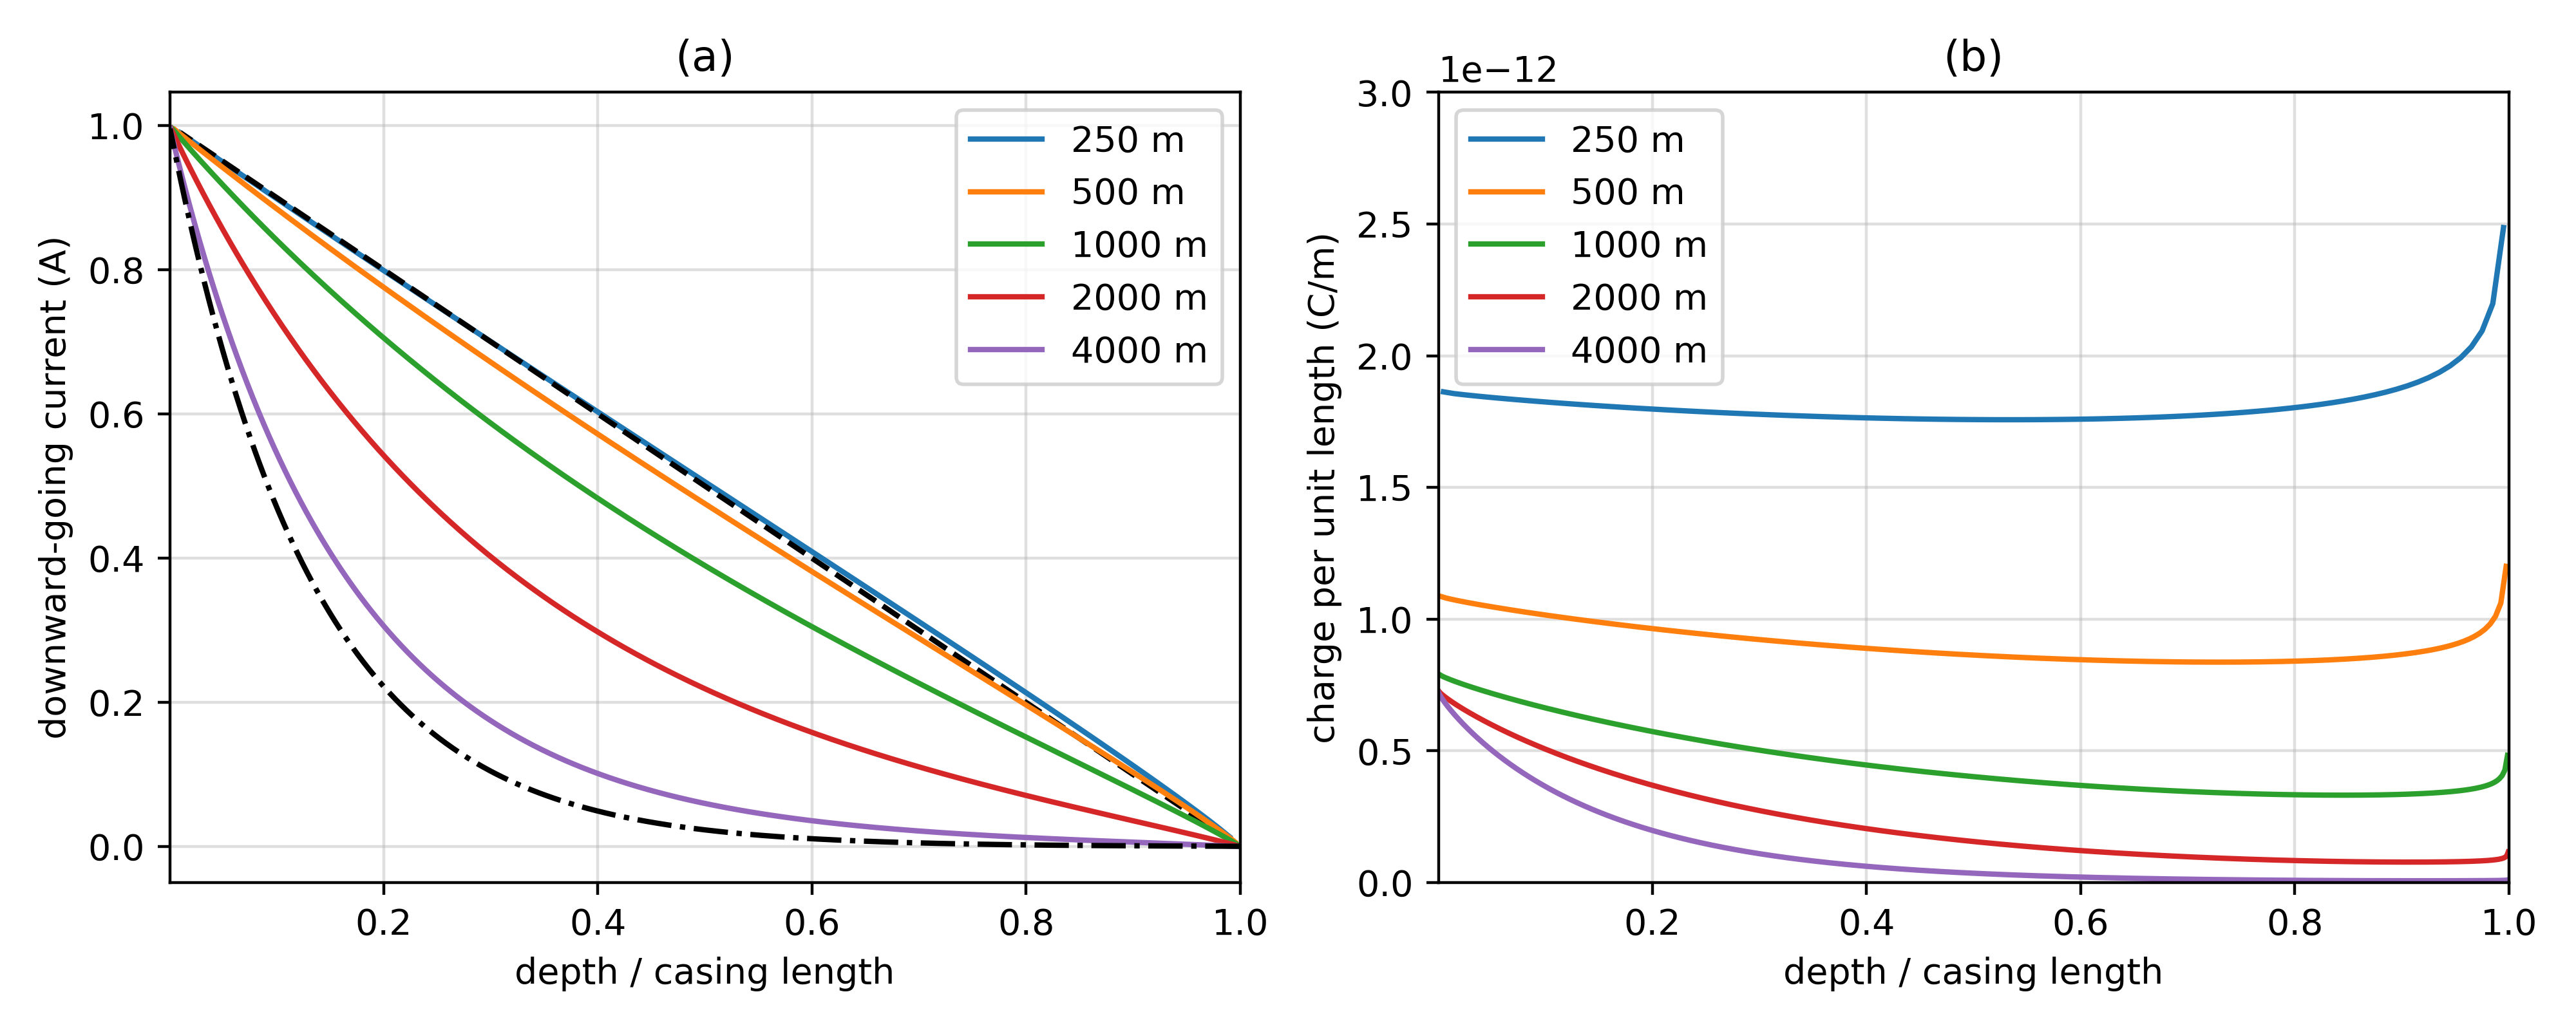
\includegraphics[width=\columnwidth]{figures/kaufman_finite_well.png}
    \end{center}
\caption{
    (a) Current along a well for 5 different wellbore lengths.
    The x-axis is depth normalized by the length of the well. The black
    dashed line shows the short-well approximation (equation 45 in \cite{Kaufman1993})
    for a 200m long well. The black dash-dot line shows the long-well approximation
    (equation 53 in \cite{Kaufman1993}) for a 4000m well.
    (b) Charge per unit length along the well for 5 different wellbore lengths.
}
\label{fig:kaufman_finite_well}
\end{figure}

\subsection{Time Domain Electromagnetics}
\label{sec:TDEM}

In this example, we examine the behaviour of electric currents in an experiment where the casing is used as an ``extended electrode''. Although the initial investigations with casings centered around using a DC source, greater information about the subsurface can be had by employing a frequency or time domain source. A particular application is the monitoring of hydraulic fracturing proppant and fluids, or CO$_2$; this is active research carried out by many groups worldwide (e.g. \cite{Hoversten2015, Um2015, Puzyrev2017, Zhang2018} among others). The challenge is to have efficient and accurate forward modelling; solving the full Maxwell equations is much more demanding than solving the DC problem. For our simulation, a positive electrode is connected to the top of the casing and a return electrode is positioned 1km away. The well has a conductivity of $10^6$ S/m and is 1km long; it has an outer diameter of 10cm and a 1cm thick casing wall. The mud which infills the well has the same conductivity as the background, $10^{-2}$ S/m. The conductivity of the air is set to $10^{-5}$ S/m; in numerical experiments, we have observed that contrasts near or larger than $\sim 10^{12}$ S/m leads to erroneous numerical solutions. For this example, we will focus on electrical conductivity only and set the permeability of the well to $\mu_0$. A step-off waveform is used, and the currents within the formation are plotted through time in Figure \ref{fig:TDEM_currents}. Panel (a) shows a zoomed-in cross section of the casing, (b) shows a vertical cross section along the line of the wire (c) shows a horizontal depth slice at 50 m depth and (d) shows a depth slice at 800 m depth. The images in panels (b), (c) and (d) are on the same color scale.

Let's start by examining Figure \ref{fig:TDEM_currents} (b), which shows the currents in the formation. The return electrode is positioned at x=1000m. At time $t=0s$, we have the DC solution. Currents flow away from the well, and eventually curve back to the return electrode. Immediately after shut-off, we see an image current develop in the formation. The image current flows in the same direction as the original current in the wire; this is opposite to currents in the formation, causing a circulation of current. The center of this circulation is visible as the null propagating downwards and to the right in Figure \ref{fig:TDEM_currents} (b). In Figure \ref{fig:TDEM_currents} (a), we see the background circulating currents being channeled into the well and propagating downwards. The depth range over which currents enter the casing depends upon time. At t=0.01 ms, the zero crossing, which distinguishes the depth between incoming and outgoing current in the casing, occurs at z=90 m, at t=0.1 ms it is at 225 m and by t=1 ms, the zero crossing approaches the midway point in the casing and is at 470m depth. At later times, the downward propagation of this null slows as the image currents are channeled into the highly conductive casing; at 5 ms it is at 520m depth, at 10ms, 560m depth and by 100ms (not shown), it is at 800m depth.

On the side of the well opposite to the wire, we also see a null develop; it is visible in the cross sections in panel (a). To help understand this, we examine the depth slices in panel (c). Behind the well, we see that as the image currents diffuse downwards and outwards, some of those currents are channeled back towards the well; this is visible in the depth slice at $10^{-4} s$. These channeled currents are opposite in direction to those the formation currents set up at t=0, which also are diffusing downwards and outwards; where these two processes intersect, there is a current shadow.

There are a number of points we feel are important about this example. The first, which has been noted by several authors (e.g. \cite{Schenkel1994, Hoversten2015}), is that the casing helps increase sensitivity to targets at depth. This occurs by two mechanisms: (1) at DC, prior to shut-off, the casing acts as an ``extended electrode'' leaking current into the formation along its length; (2) after shut-off, it channels the image currents and increases the current density within the vicinity of the casing. The second point to note is that there are several survey design considerations raised by examining the currents: targets that are positioned where there is significant current will be most illuminated. If the target is near the surface and offset from the well, a survey where the source wire runs along the same line as the target will have the added benefits of the excitation due to the image currents. These benefits are twofold: (1) the passing image-current increases the current density for a period of time, and (2) the changing amplitude and direction of the currents with time generate different excitations of the target. this should provide enhanced information in an inversion, as compared to a single excitation that is available from a DC survey. For deeper targets in this experiment, the passing image current has diffused significantly, and thus it appears that the wire location has less impact on the magnitude of the current density with location. However, it is possible that increasing the wire-length could be beneficial. This extension is straightforward and could be examined with the provided script. There may also be added benefit by having the target positioned along the same line as the source wire, as at later times, the direction of current reverses, changing the excitation of the target.. The final point to note from this example is that although this is a simple model, the behavior of the currents is not intuitive; visualizations of the currents, fields and fluxes, particularly when connected with the interactive Jupyter computing environment \citep{Perez2015}, allow researchers to explore the basic physics and prompts new questions. Such simulations and visualizations have proved valuable in the context of geoscience education \citep{Oldenburg2017} and can be a useful tool for understanding the physical processes that contribute to the data we observe.



\begin{figure}
    \begin{center}
    \includegraphics[width=0.95\columnwidth]{figures/casing_software/TDEM_currents.png}
    \end{center}
\caption{
    Current density for a time domain experiment where one electrode is connected to the top of the casing and a return electrode is on the surface, 1000 m away.
    Six different times are shown, corresponding to each of the six rows; the times are indicated in the plots in panel (d).
    Panel (a) shows a zoomed-in cross section of the current density in the immediate vicinity of the steel cased well.
    Panel (b) shows a cross section through the half-space along the same line as the source wire.
    Panels (c) and (d) show depth-slices of the currents at 54 m and 801 m depth.
}
\label{fig:TDEM_currents}
\end{figure}


\subsection{Frequency Domain Electromagnetics}
\label{sec:FDEM}

In the DC example, we discussed how charges are distributed along the well and currents flow into the formation. The time domain example extended the analysis of grounded sources, showed the potential importance of EM induction effects and illuminated the underlying physics. From a historical perspective, however, practical developments in EM were pursued in the frequency domain; the mathematics is more manageable in the frequency domain, and technological advances were being made in the development of induction well-logging tools \citep{Doll1949, Moran1962}. Although conductivity of the pipes is generally plays the most dominant role in attenuating the signal, the magnetic permeability is non-negligible \citep{Wait1977}; it is the product of the conductivity and permeability that appears in the description of EM attenuation. Also, the fact that permeable material becomes magnetized in the presence of an external field complicates the problem.
\cite{Augustin1989} is one of the first papers on induction logging in the presence of steel cased wells that aims to understand and isolate the EM response of the steel cased well. Using a combination of scale modelling and analytical mathematical modelling, they examine the impacts of conductivity and magnetic permeability on the magnetic field observed in the pipe. In the two following examples we attempt to unravel this interplay between conductivity and magnetic permeability.


\subsubsection{Example 1: Comparison with scale model results}

The first experiment they discuss is a scale model using two different pipes, a conductive copper pipe and a conductive, permeable iron pipe; each pipe is 9m in length. The copper pipe had an inner diameter of 0.063m and a thickness of 0.002m, while the iron pipe had a 0.063m inner diameter and 0.0043m wall thickness. A source-loop, with radius 0.6m was co-axial with the pipe and in one experiment positioned at one end of the pipe (which they refer to as the ``semi-infinite pipe'' scenario). In another experiment the source loop is positioned at the midpoint of the pipe (which they refer to as the ``infinite pipe'' scenario); for both experiments, magnetic field data are measured as a function of frequency at the central axis of the pipe. Their results are presented in terms of a Field Strength Ratio (FSR), which is the ratio of the absolute value of the magnetic field at the receiver with the absolute value of the magnetic field if no pipe is present (Figure 3 in \cite{Augustin1989}). At low frequencies, for the data collected within the iron pipe, static shielding (FSR $<$ 1) was observed for the measurements where the receiver was in the plane of the source loop for both the ``infinite'' and ``semi-infinite'' scenarios. When the receiver was positioned within the pipe, 1.49m offset from the plane of the source loop, static enhancement effects (FSR $>$ 1) were observed for both the infinite and semi-infinite scenarios. Using this experiment for context, we will compare the behaviour of our numerical simulation with the observations in \citep{Augustin1989} and examine the nature of the static shielding and enhancement effects.

For our numerical setup, the pipes are 9m in length and have an inner diameter of 0.06m. The copper pipe has a casing-wall thickness of 0.002m and the iron pipe has a thickness of 0.004m. Following the estimated physical property values from \cite{Augustin1989}, we use a conductivity of $3.5 \times 10^7$ S/m and a relative permeability of 1 for the copper pipe. For the iron pipe, a conductivity of $8.0 \times 10^6$ S/m and a relative permeability of 150 is used. A background conductivity of $10^4 ~\Omega$m is assumed. The computed FSR values for the axial magnetic field as a function of frequency are shown in Figure \ref{fig:AugustinFSR}.


\begin{figure}
    \begin{center}
    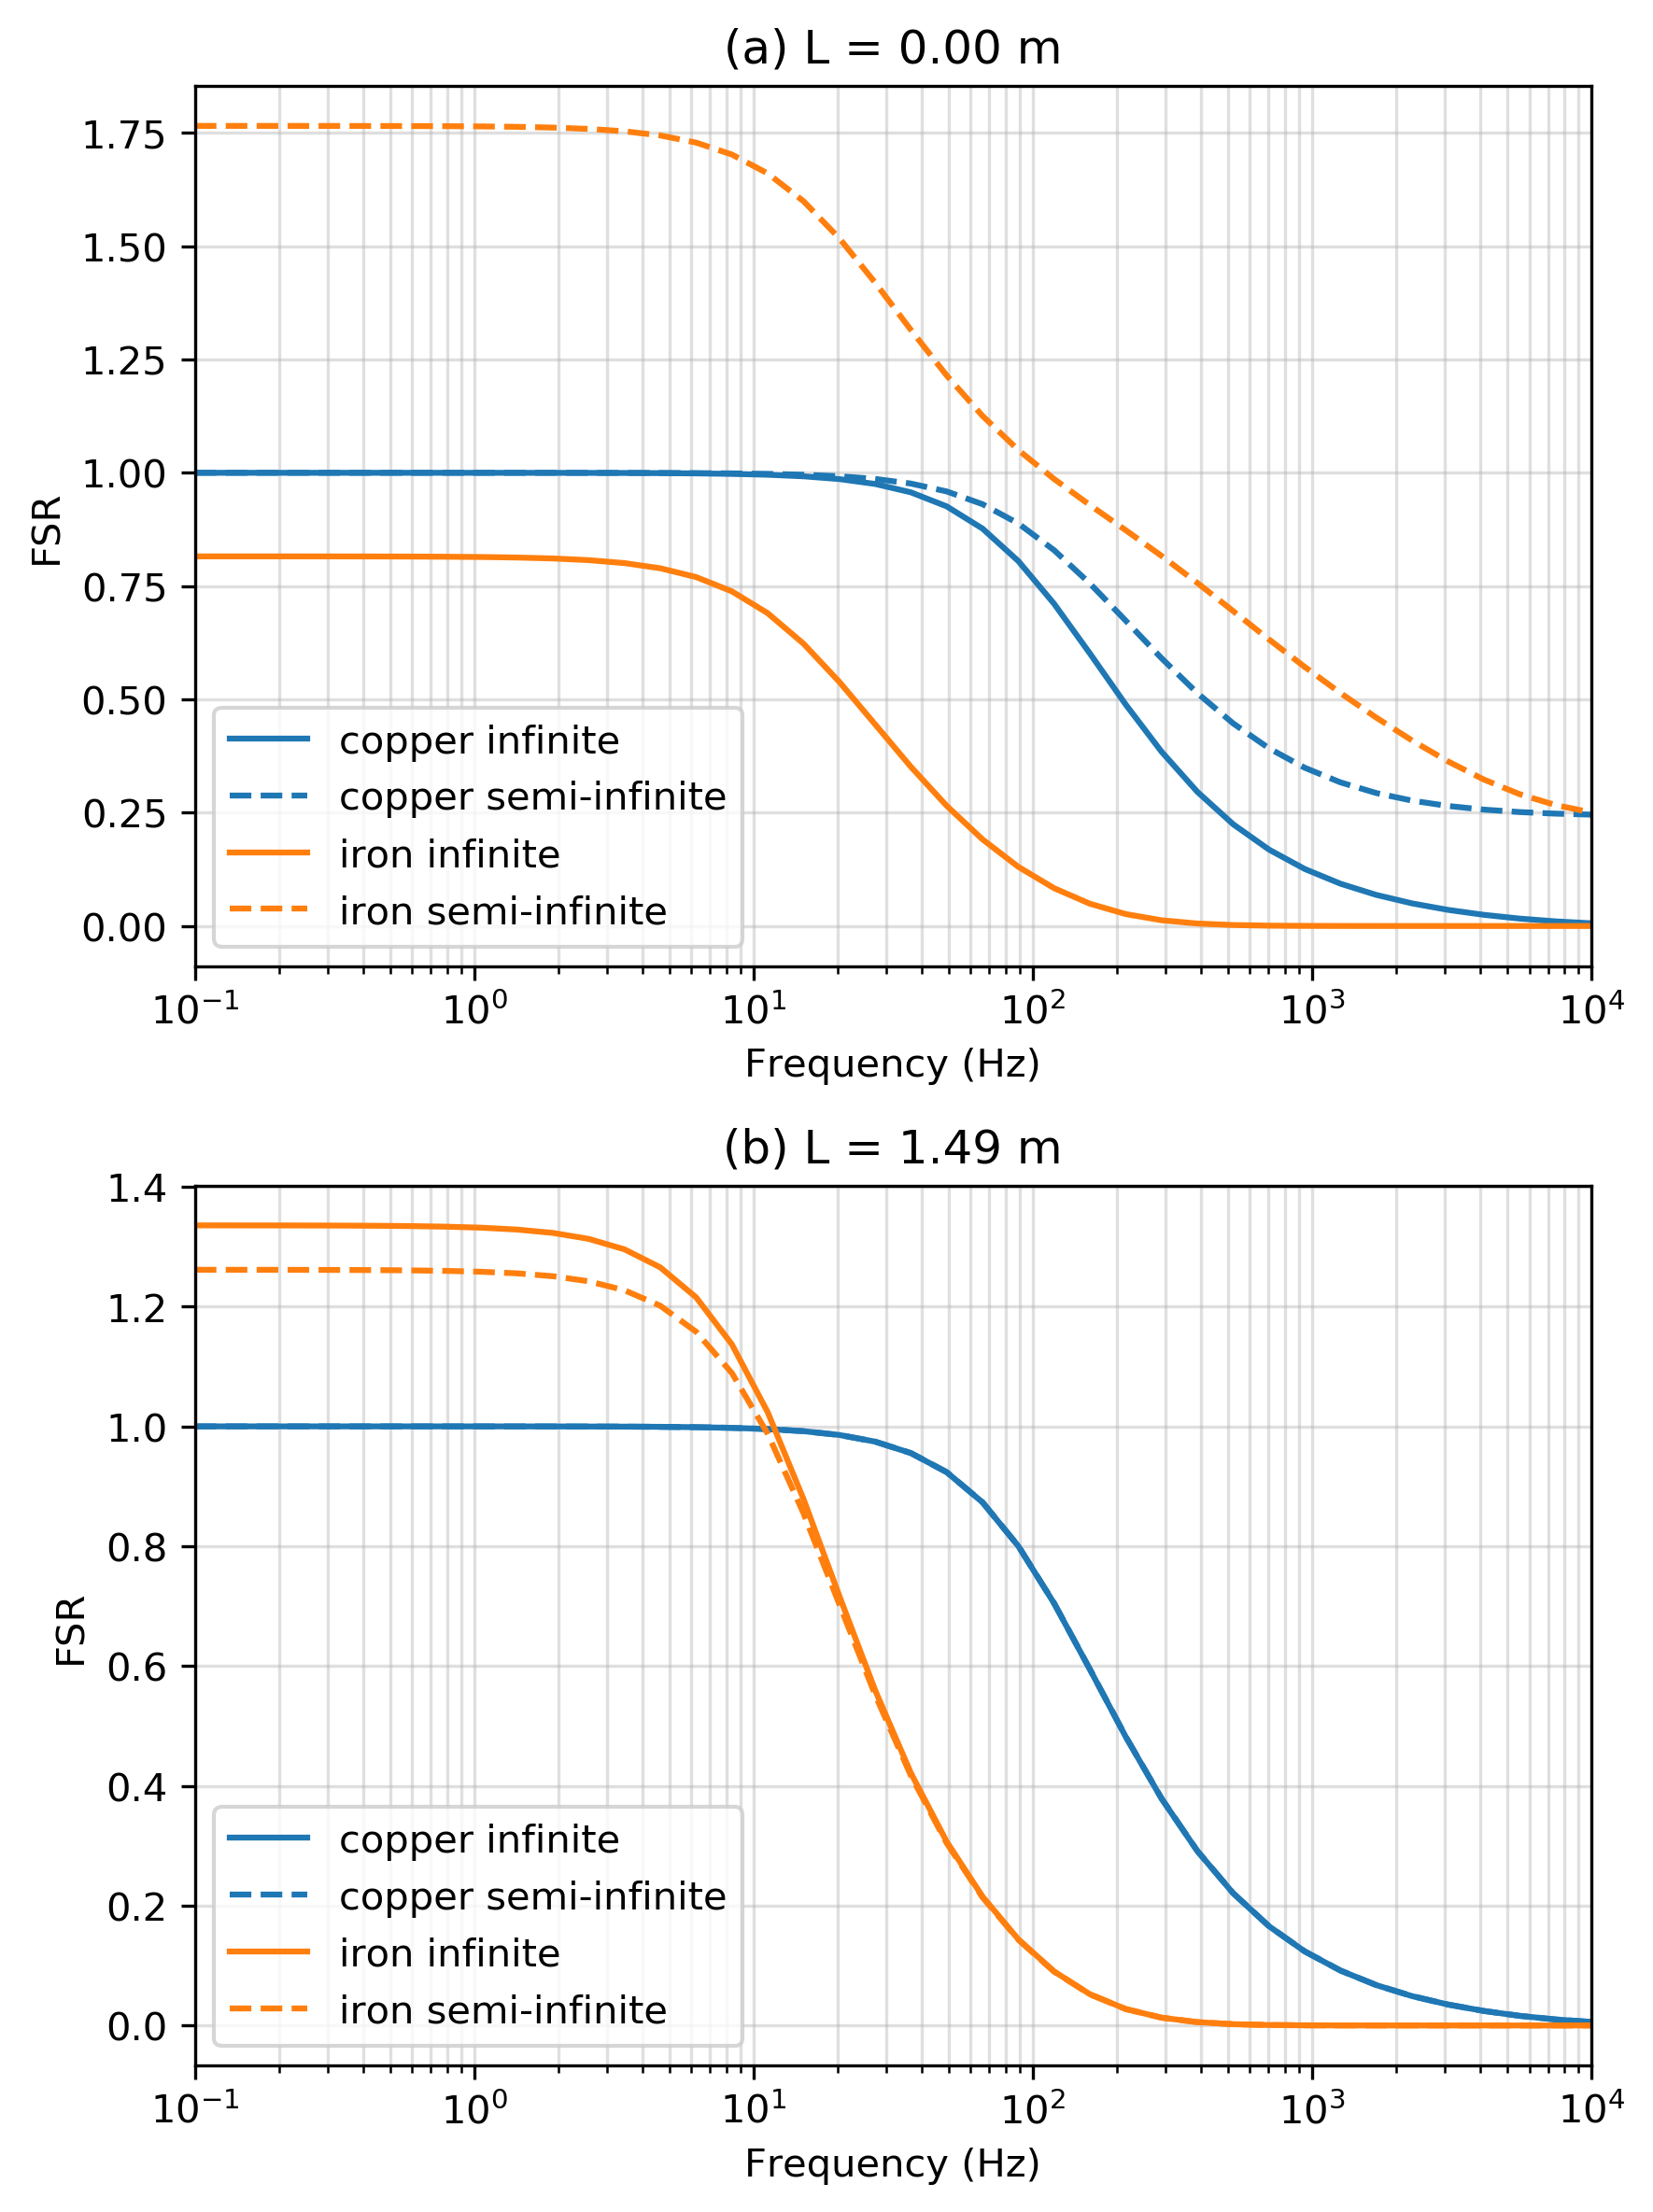
\includegraphics[width=0.6\columnwidth]{figures/casing_software/AugustinFSR.png}
    \end{center}
\caption{
    Field strength ratio (FSR), the ratio of the measured vertical magnetic field with the free space magnetic field, as a function of frequency for two different reciever locations.
    In (a), the reciever is in the same plane as the source, in (b), the reciever is 1.49m offset from the source.
}
\label{fig:AugustinFSR}
\end{figure}


Let's start by examining the response of the conductive pipe. At low frequencies, the FSR for the copper pipe (blue lines) is 1 for both the infinite (solid line) and semi-infinite (dashed line) scenarios, as the field inside the copper pipe is equivalent to the free-space field. With increasing frequency, eddy currents are induced in the pipe which generate a magnetic field that opposes the primary, causing a decrease in the observed FSR. When the source and receiver are in the same plane (L=0.00m), the rate of decrease is more rapid in the infinite scenario than the semi-infinite. Since there is conductive material on both sides of the receiver in the infinite case, we would expect attenuation of the fields to occur more rapidly than in the semi-infinite case. This observation is consistent with Figure 3a in \cite{Augustin1989}. For the offset receiver (L=1.49m), they observed a slight separation in the infinite and semi-infinite curves which we do not; however, they attributed this to potential errors in magnetometer position. Thus, overall, the numerical results for the copper pipe are in good agreement with the scale model results observed by \cite{Augustin1989}.

Next, we examine the response of the conductive, permeable pipe. In Figure \ref{fig:AugustinFSR}b, we observe a static enhancement effect (FSR $>$ 1) at low frequencies. The enhancement is larger in the infinite scenario than the semi-infinite scenario; this is in agreement with Figure 3b in \cite{Augustin1989}. There is however, a significant discrepancy between our numerical simulations and the scale model for the semi-infinite pipe when the source and receiver lie in the same plane(Figure \ref{fig:AugustinFSR}a). \cite{Augustin1989} observed a static shielding effect for both the infinite and semi-infinite scenarios, whereas we observe a static shielding for the infinite scenario, but a significant static enhancement for the semi-infinite case. To examine what might be the cause of this, we will examine the magnetic flux density in this region of the pipe.

In Figure \ref{fig:AugustinBfields}, we have plotted: (a) the secondary magnetic flux in the infinite-pipe scenario near the source (z=-4.5m), (b) the secondary magnetic flux in the semi-infinite scenario (z=0m for the source), and (c) top 5cm of the semi-infinite pipe. All plots are at 0.1Hz. The primary magnetic field is directed upwards within the regions we have plotted, so upward-going magnetic flux indicates a static enhancement effect, and downward-oriented magnetic flux indicates static shielding effects. In (a) we see a transition between the static shielding in the vicinity of the source to a static enhancement approximately 0.5m above and below the plane of the source. Similarly in (b), we notice a sign-reversal in the z-component of the secondary magnetic flux at a depth of 0.6m. These behaviours are quite comparable to Augustin et al.'s observation of a transition from shielding to enhancement occurring at distances greater than 0.8m from the source. Numerical experiments show that the vertical extent of the region over which static shielding is occuring increases with increasing pipe diameter, and similarly increases with increasing loop radius while the magnitude of the effect decreases. This can be understood by considering how the pipe is magnetized; for a small loop radius, the magnetization is largely localized near the plane of the source and rapidly falls off with distance from the plane of the source. Localized, large amplitude magnetization causes the casing to act as a collection of dipoles around the circumference of the casing. As the radius of the loop increases, the magnetization spreads out along the length of the well resulting in longer, lower-amplitude dipoles, thus both increasing the extent of the region over which static shielding is occuring as well as decreasing its amplitude.


\begin{figure}
    \begin{center}
    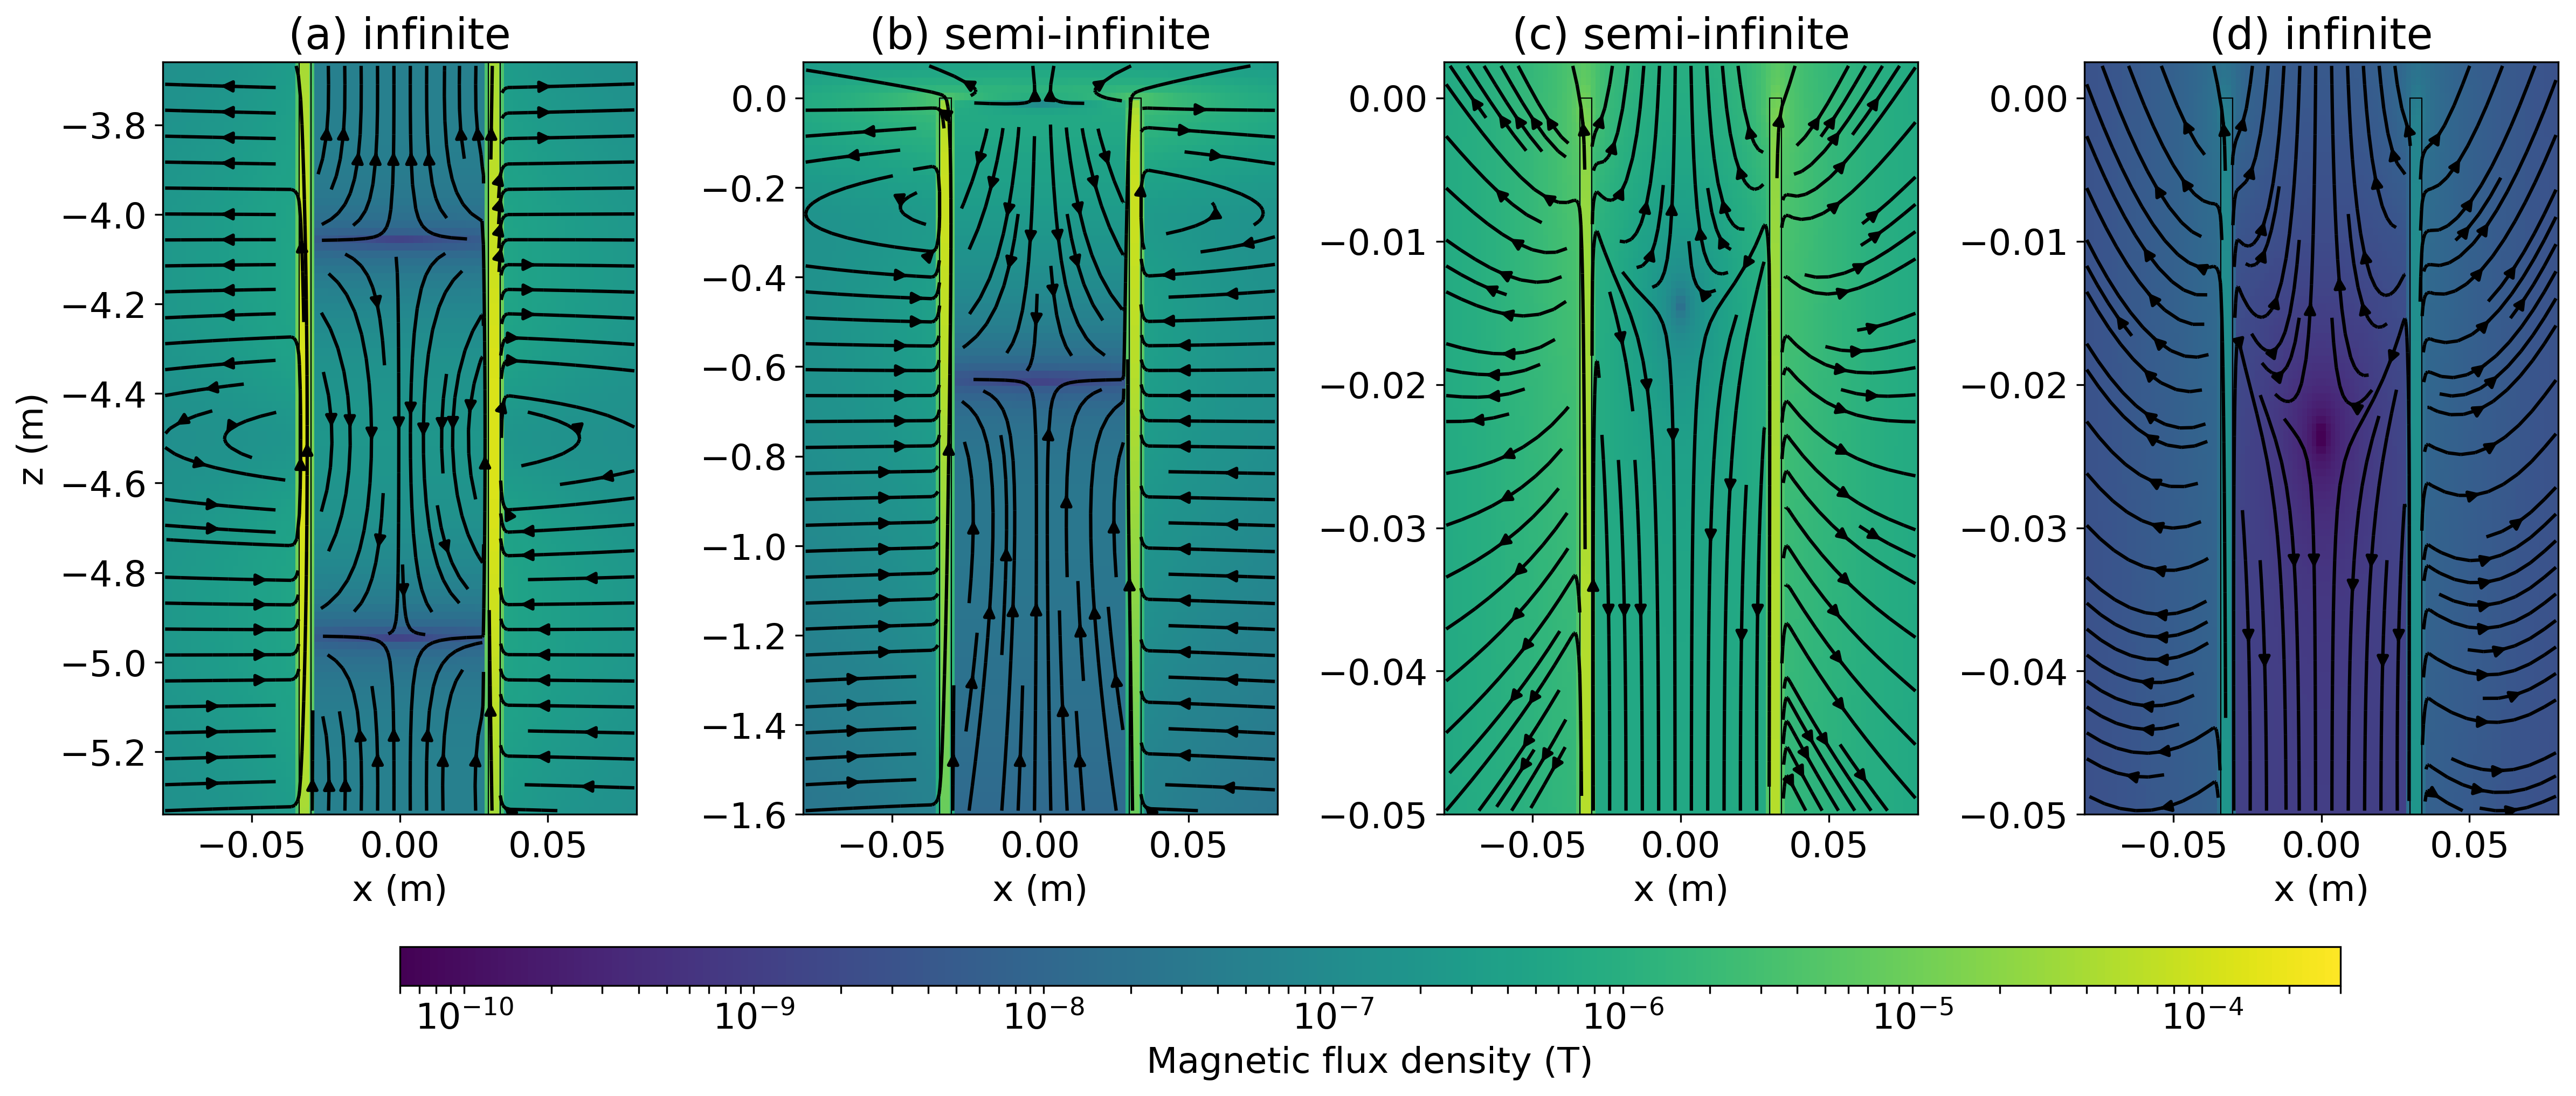
\includegraphics[width=\columnwidth]{figures/casing_software/AugustinBfields.png}
    \end{center}
\caption{
    Magnetic flux density at 0.1 Hz in the region of the pipe near the plane of the source for
    (a) the ``infinite'' pipe, where the source is located at -4.5 m and the pipe extends from 0 m to -9 m,
    (b) a ``semi-infinite'' pipe, where the source is located at 0 m and the pipe extends to -9 m.
    In (c), we zoom in to the top 5 cm of the ``semi-infinite'' pipe,
    and (d) shows the 5 cm at the top-end of the ``infinite'' pipe.
}
\label{fig:AugustinBfields}
\end{figure}


This explains the nature of the static enhancement and static shielding effects, but to explain the discrepancy between the static shielding observed in the semi-infinite pipe when L=0m by Augustin et al., and the static enhancement we observe in Figure \ref{fig:AugustinFSR}a, we examine the magnetic flux density in the top few centimeters of the pipe. Figure \ref{fig:AugustinBfields}c shows the top 5cm of the secondary magnetic flux in the semi-infinite pipe; the source is in the z=0m plane.  Zooming in reveals there is yet another sign reversal near the end of the pipe. This is evident even in the infinite-pipe scenario (Figure \ref{fig:AugustinFSR}d), where the source is offset by several meters from the end of the pipe. This edge-effect perhaps bears some similarities to what we observed in Figure \ref{fig:kaufman_finite_well}b, where we saw a build up of charge near the end of the pipe in the DC scenario. At the end of the pipe, we encounter the situation where the normal component of the flux ($\vec{j}, \vec{b}$) from the pipe to the background needs to be continuous both in the radial and vertical directions at the end of the pipe as does the tangential component of the fields ($\vec{e}, \vec{h}$). The interplay of these two constraints at the end of the pipe results in more complexity in the resultant fields and fluxes. Within the span of a few centimeters we transition from static enhancement at the top of the pipe to a static shielding further down. An error as small as a few centimeters in the position of the magnetometer causes a reversal in behavior; in Figure \ref{fig:Augustin3cm}, we have plotted the FSR for a magnetometer positioned 3cm beneath the plane of the source, and the static-shielding behavior observed for the semi-infinite pipe is much more aligned with that observed in Figure 3a in \cite{Augustin1989}.



\begin{figure}
    \begin{center}
    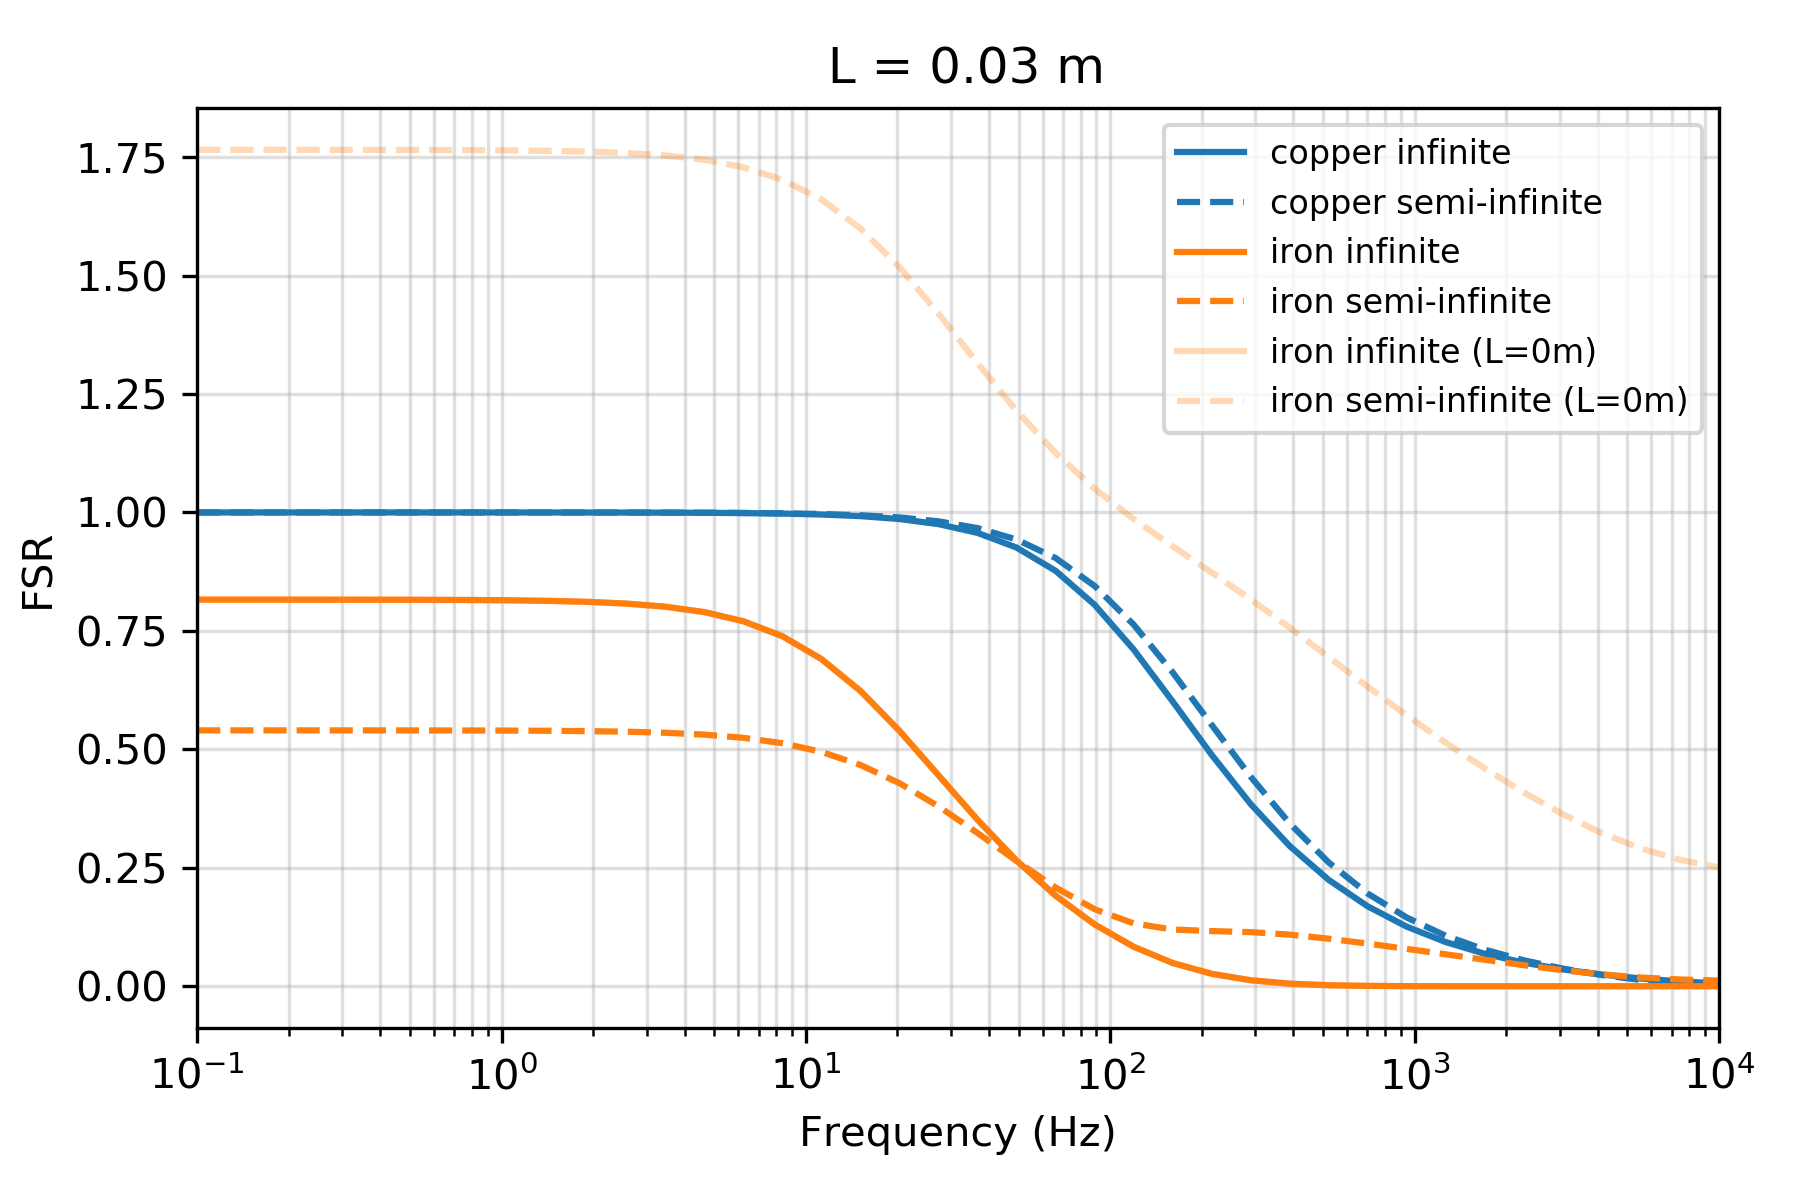
\includegraphics[width=0.6\columnwidth]{figures/Augustin3cm.png}
    \end{center}
\caption{
    Field strength ratio, FSR, for a reciever positioned 3cm beneath
    the plane of the source. For comparison, we have plotted the
    FSR for the permeable pipe when the source and reciever lie in the same
    plane (L=0.00m) with the semi-transparent orange lines.
    Note that the infinite-pipe solutions for L=0.03m and L=0.00m overlap.
}
\label{fig:Augustin3cm}
\end{figure}



These experiments revealed some insights into the complexity of the fields within the pipe and illustrated the role of permeability in the character of the responses at low frequency. Next, we move to larger scales and examine the role of conductivity and permeability in the responses we observe in the borehole.

\subsubsection{Example 2: Conductivity and permeability in the inductive response of a well}

We consider a 2km long well with an outer diameter of 10cm and thickness of 1cm in a whole-space which has a resistivity of $10^4$ $\Omega$m. A loop with radius 100m is coaxial with the well and positioned at the top-end of the well. A receiver measuring the z-component of the magnetic flux density is positioned 500 m below the transmitter loop, along the axis of the well. We will examine both time-domain and frequency-domain responses.

In electromagnetics, it is often the product of permeability and conductivity that we consider to be the main controlling factor on the EM responses. To examine the contribution of each to the measured responses, we will examine two scenarios. In the first, the well has a conductivity of $10^8$ S/m and a relative permeability of 1, and in the second, the well has a conductivity of $10^6$ S/m and a relative permeability of 100; thus the product of conductivity and permeability is equivalent for both wells.

Similar to the analysis done by \cite{Augustin1989} when looking at the role of borehole radius in the behaviour of the magnetic response (e.g. figure 8), we will examine the normalized secondary field (NSF) which is the ratio of the secondary field with the amplitude of the primary. The primary is defined to be the free-space response. In Figure \ref{fig:fdemNSF}, we have plotted the normalized secondary field for the two pipes considered, the conductive pipe (blue) and the conductive, permeable pipe (orange). Let's start by examining the conductivity response in Figure \ref{fig:fdemNSF}. Where the value of the NSF is zero, the primary dominates the response; this is the case at low frequencies where induction is not yet contributing to the response. As frequency increases, currents are induced in the pipe which generate a secondary magnetic field that opposes the primary, hence the NSF becomes negative. When the real part of the NSF (solid line) is -1, the secondary magnetic field is equal in magnitude but opposite in direction to the free-space primary and the measured real field is zero. Values less than -1 indicate a sign reversal in the real magnetic field. Similarly, when the imaginary part of the response function goes above zero, there is a sign reversal in the imaginary component. Note that these sign reversals occur even in a half-space and are a result of sampling the fields within a conductive medium; in this case the receiver was 500m below the surface.

As compared to the conductive pipe, the frequency at which induction sets in is higher for the conductive, permeable pipe. We also notice that the amplitude variation of both the imaginary and real parts is larger for the permeable pipe. To examine the contribution of conductivity and permeability to the responses, we have plotted the real part of the secondary magnetic flux density, $\mathbf{b}$, in Figure \ref{fig:bfdem}. The top row shows the response within the conductive pipe and the bottom row shows the conductive, permeable pipe. The primary magnetic flux is oriented upwards and we can see that all of the secondary fields generated are oriented downwards. Similar to the previous example, we see that at low frequencies, there is magnetostatic response due to the permeable pipe. However, due to the larger length scales of the source loop and the casing in this example, there is no measurable contribution at the receiver. At 1Hz, we can see that induction is starting to contribute to the signal for the conductive pipe, while for the permeable pipe, it is not until $\sim$10 Hz that we begin to observe the contribution of induction. At 100 Hz, the secondary magnetic field is stronger in amplitude than the primary, and the NFS is less than -1 for both the conductive and permeable pipes. The amplitude of the secondary within the permeable pipe is stronger than that in the conductive pipe. At 1000 Hz, we have reached the asymptote of NSF=-1 for both the conductive and permeable pipes; the secondary magnetic flux is equal in magnitude but opposite in direction to the primary.

\begin{figure}[htb]
    \begin{center}
    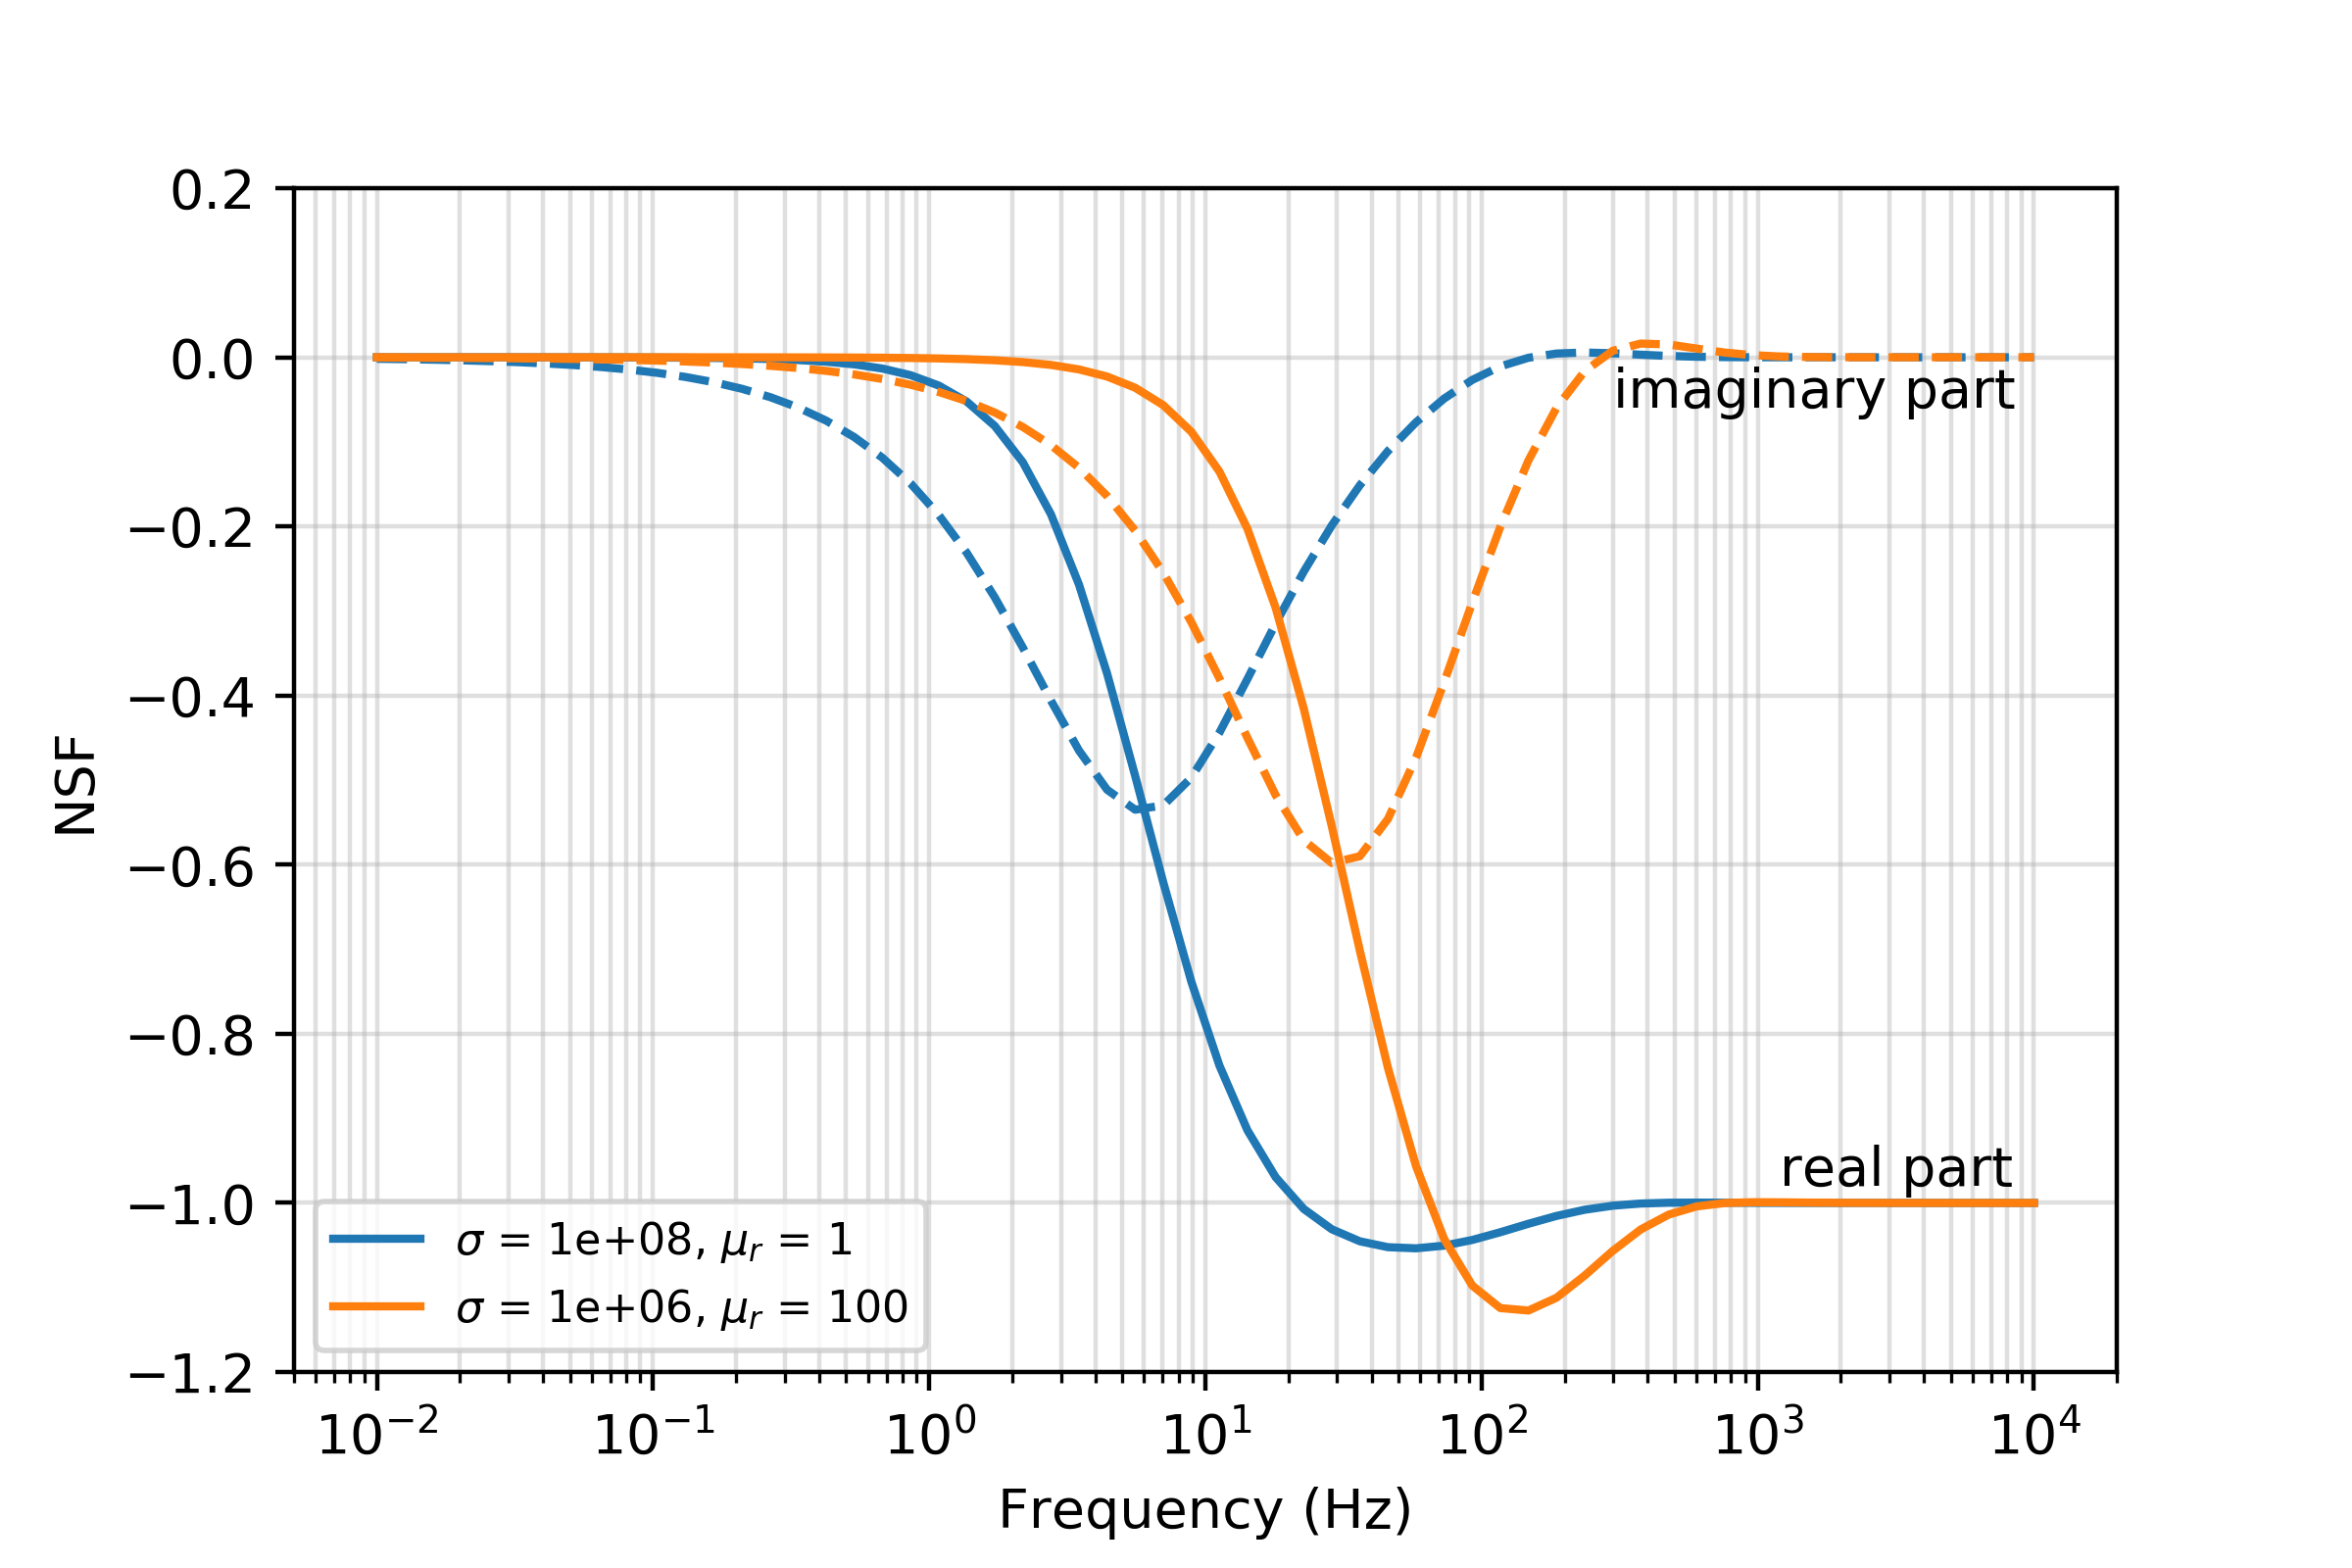
\includegraphics[width=0.6\columnwidth]{figures/casing_software/fdemNSF.png}
    \end{center}
\caption{
    Normalized secondary field, NSF, as a function of frequency for two wells.
    The NSF is the ratio of the secondary vertical magnetic field with the primary magnetic field at the receiver location ($z=$-500 m);
    the primary is defined as the whole-space primary.
}
\label{fig:fdemNSF}
\end{figure}



\begin{figure}
    \begin{center}
    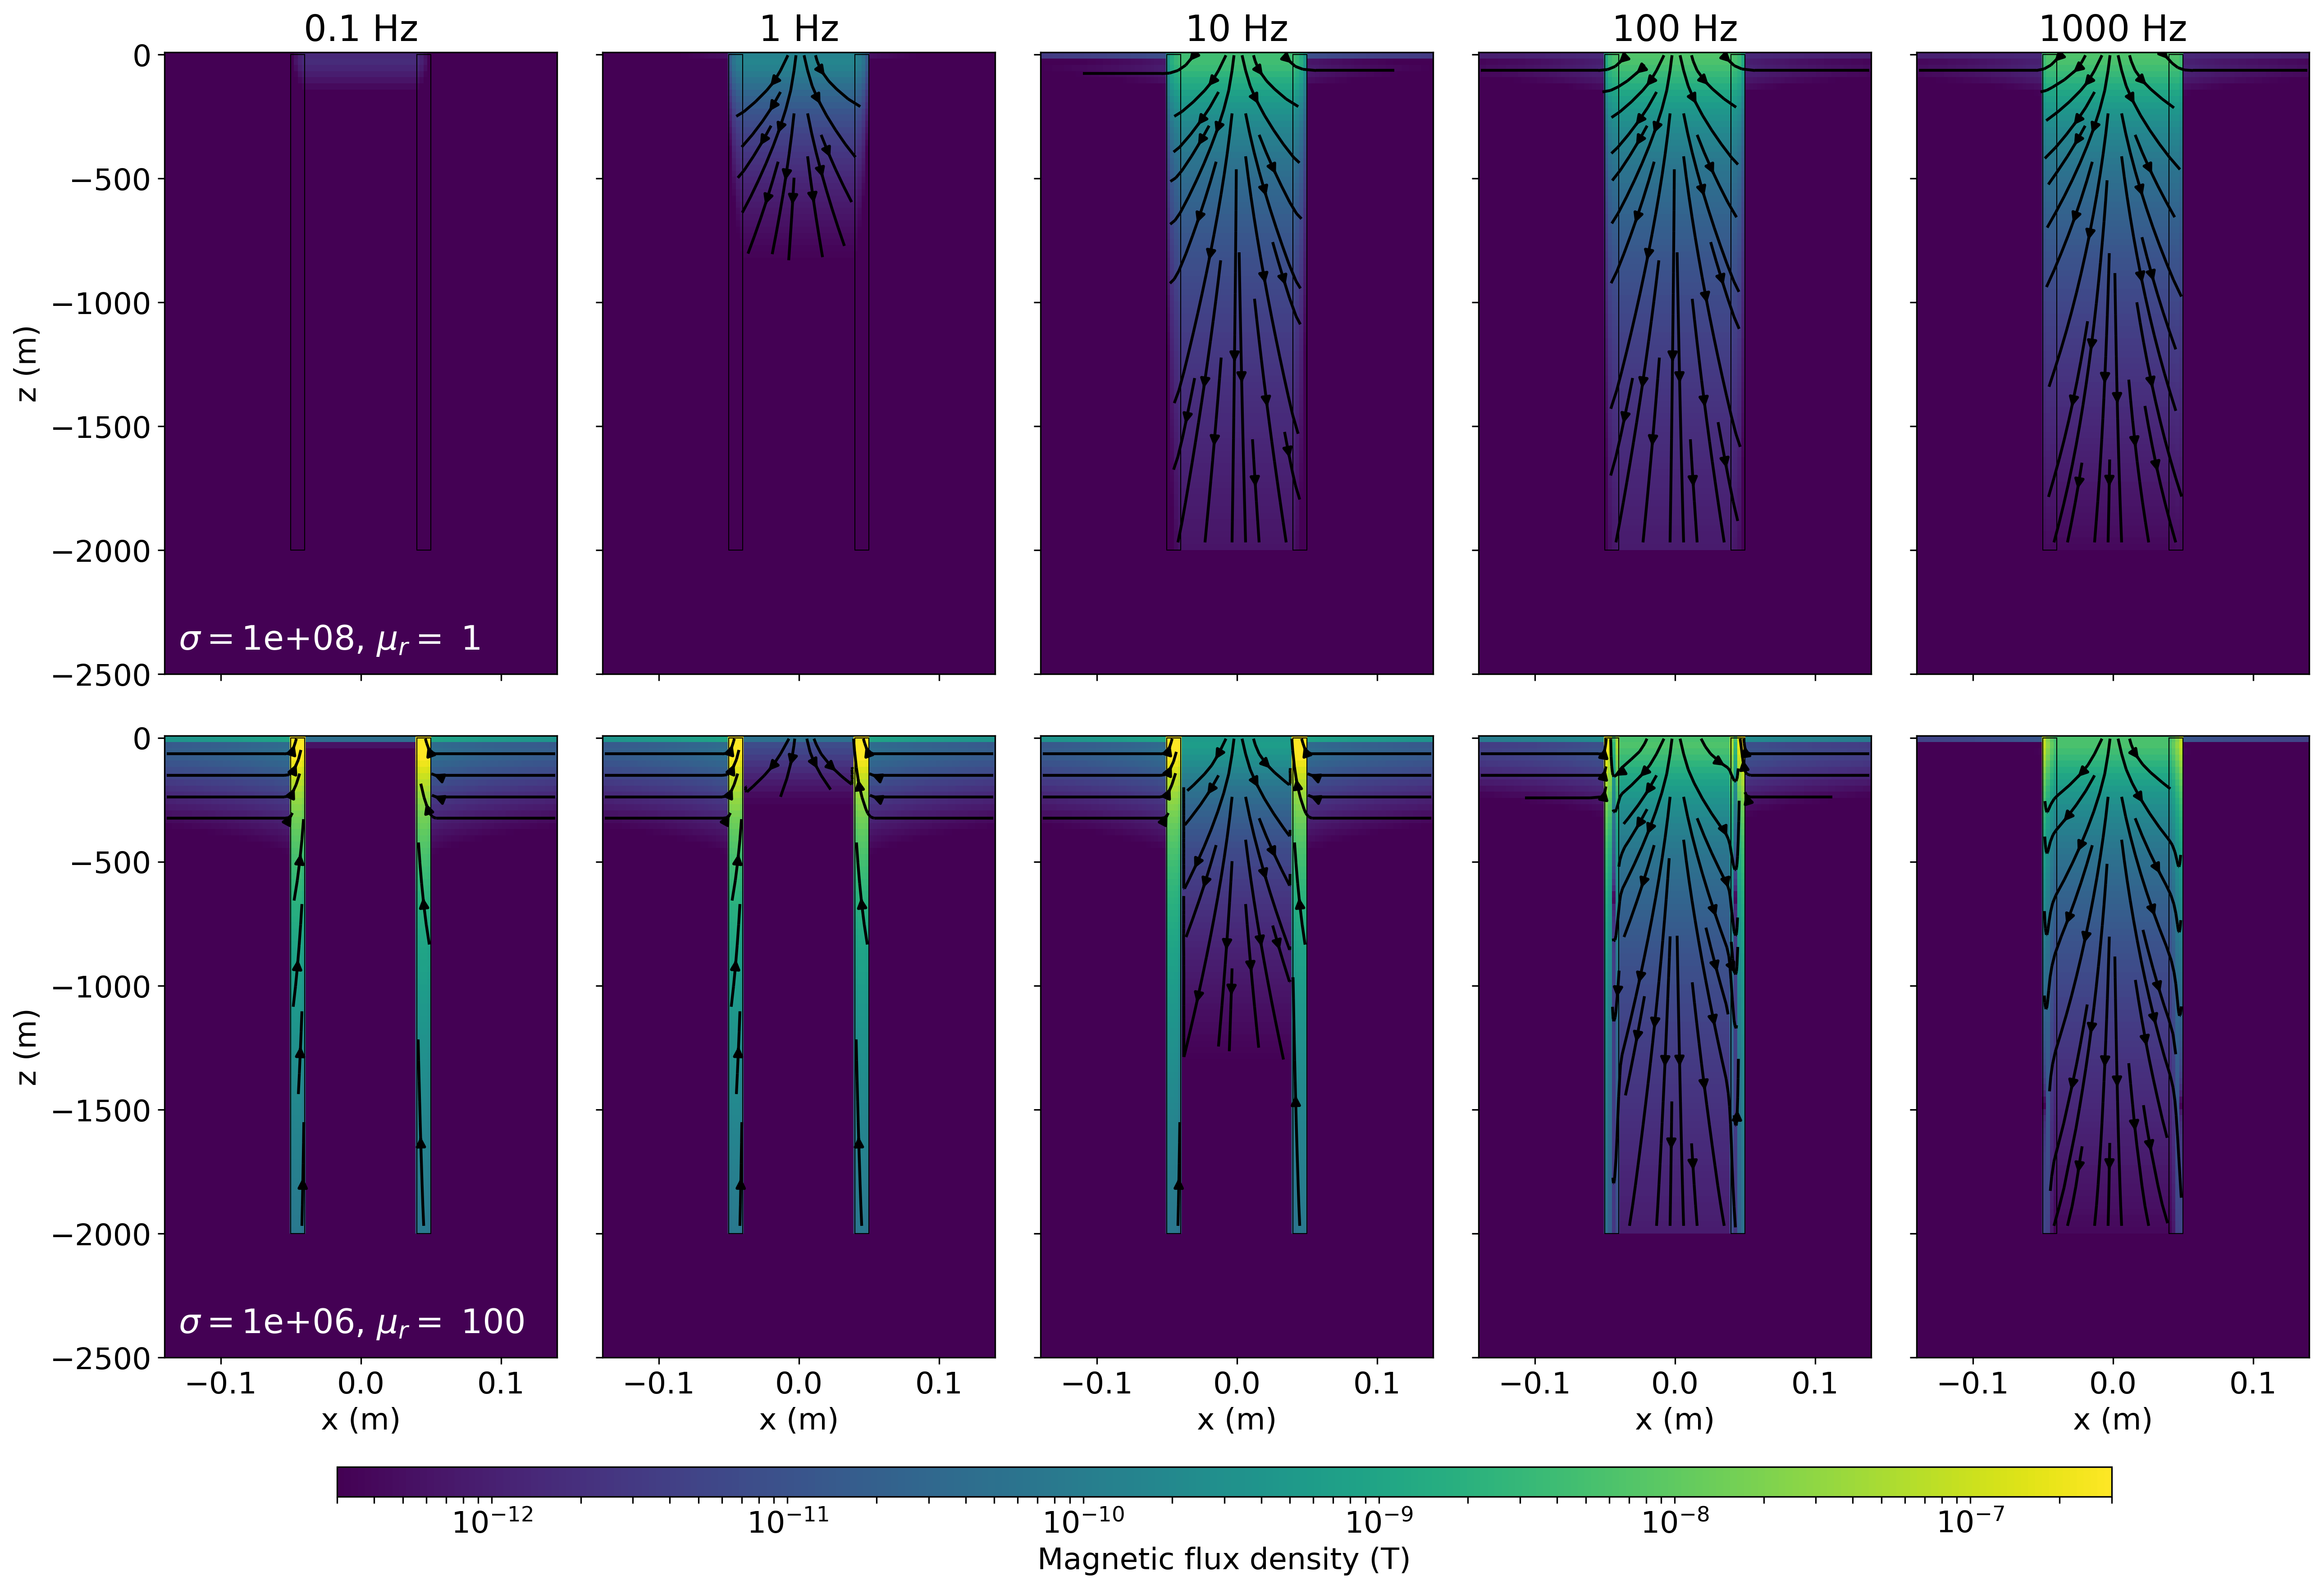
\includegraphics[width=\columnwidth]{figures/bfdem.png}
    \end{center}
\caption{
    Secondary magnetic flux density (with respect to a whole-space primary) at five different frequencies for a conductive pipe (top row)
    and for a conductive, permeable pipe (bottom row).
}
\label{fig:bfdem}
\end{figure}



Conducting a similar experiment in the time-domain, we can compare the responses as a function of time. For this experiment, a step-off waveform is employed and data are measured after shut-off, the NSF is plotted in Figure \ref{fig:tdemNSF}. Note here that the secondary field is in the same direction as the primary, so after the source has been shut off, the secondary field is oriented upwards, as shown in Figure \ref{fig:btdem}. Shortly after shut-off, the rate of increase in the secondary field is the same for both the conductive and the conductive, permeable wells. A maximum normalized field strength of approximately 1 is reached for both cases. The responses begin to differ at $10^{-3}$ s where the conductive well maintains a NFS $\sim 1$ for approximately 1ms longer than the permeable well before the fields decay away.


\begin{figure}[htb]
    \begin{center}
    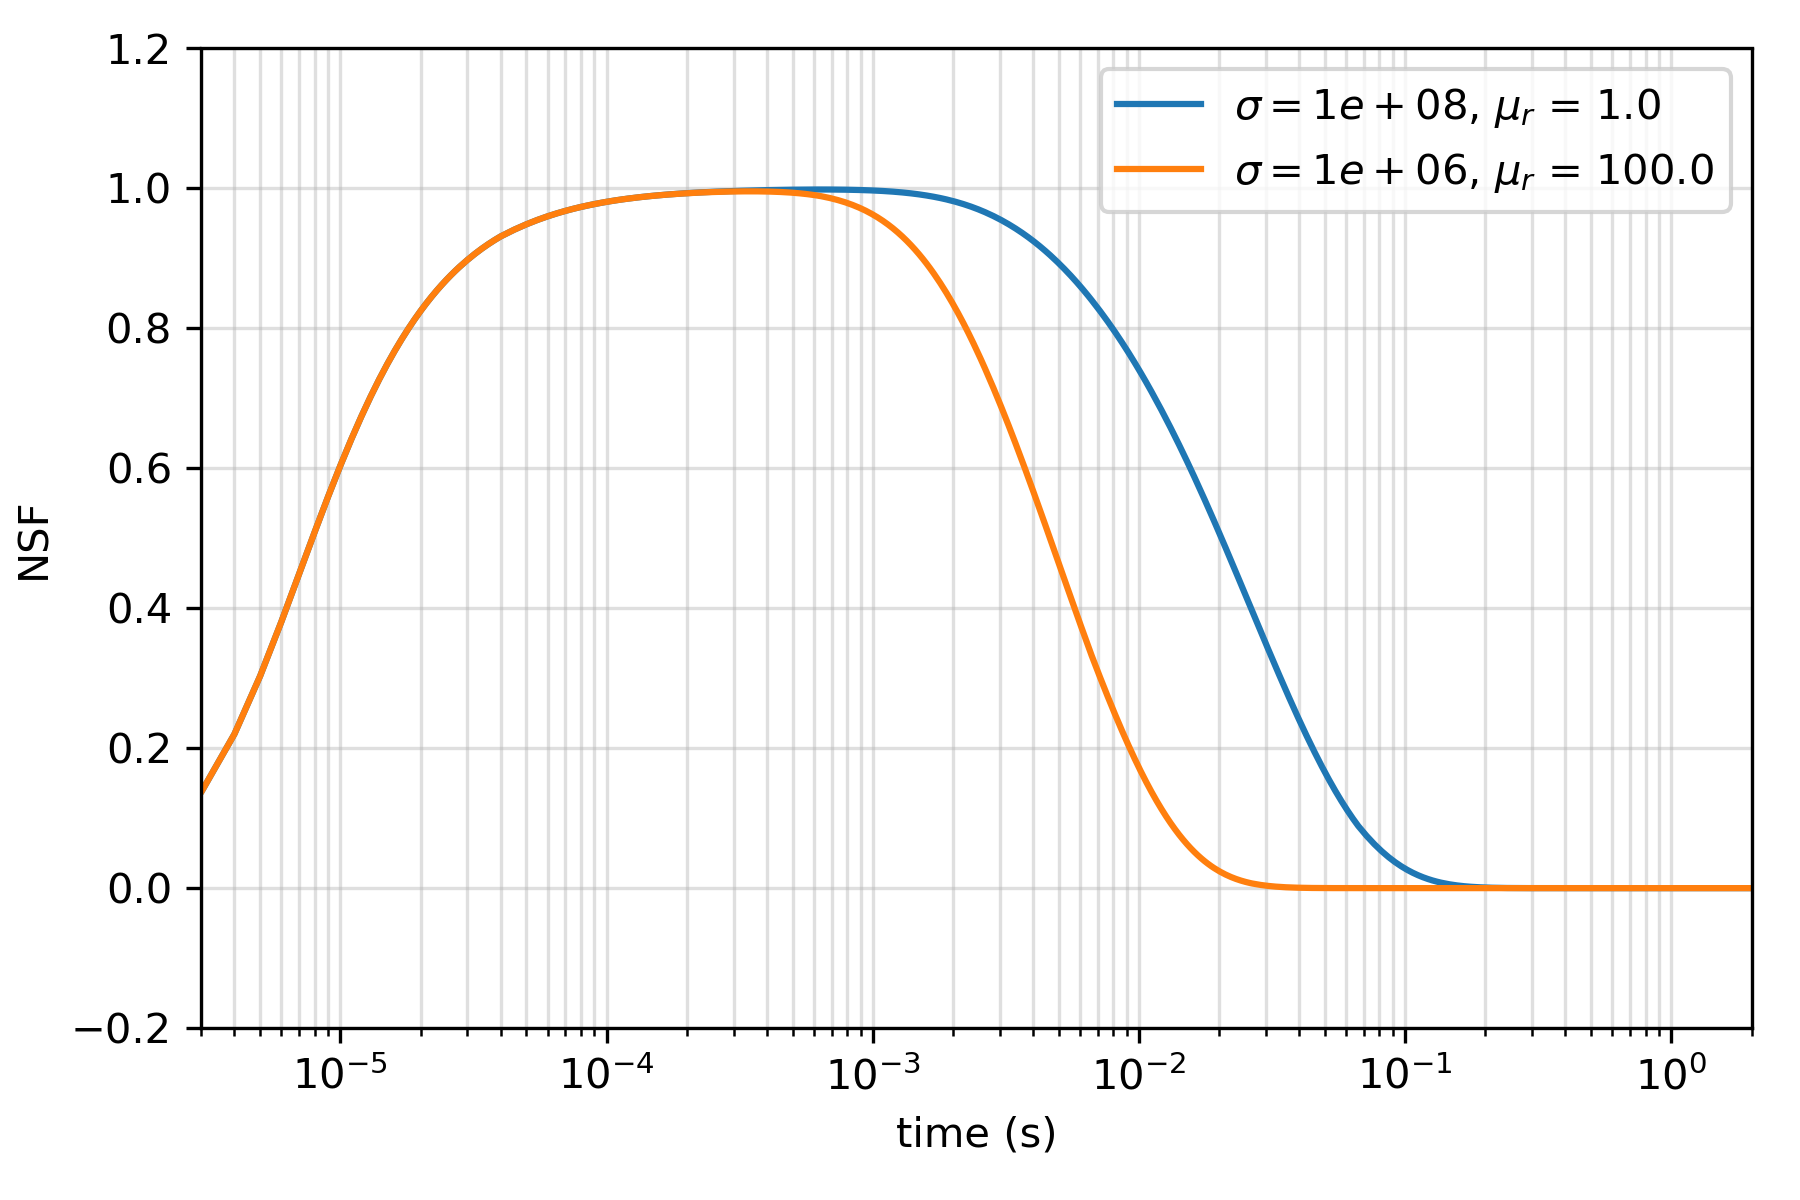
\includegraphics[width=0.6\columnwidth]{figures/tdemNSF.png}
    \end{center}
\caption{
    Normalized secondary field (NSF) through time.
    In the time-domain, we compute the NSF by taking the difference between the total magnetic flux at the reciever and the whole-space response
    and then taking the ratio with the whole-space magnetic flux prior to shutting off the transmitter.
}
\label{fig:tdemNSF}
\end{figure}



\begin{figure}
    \begin{center}
    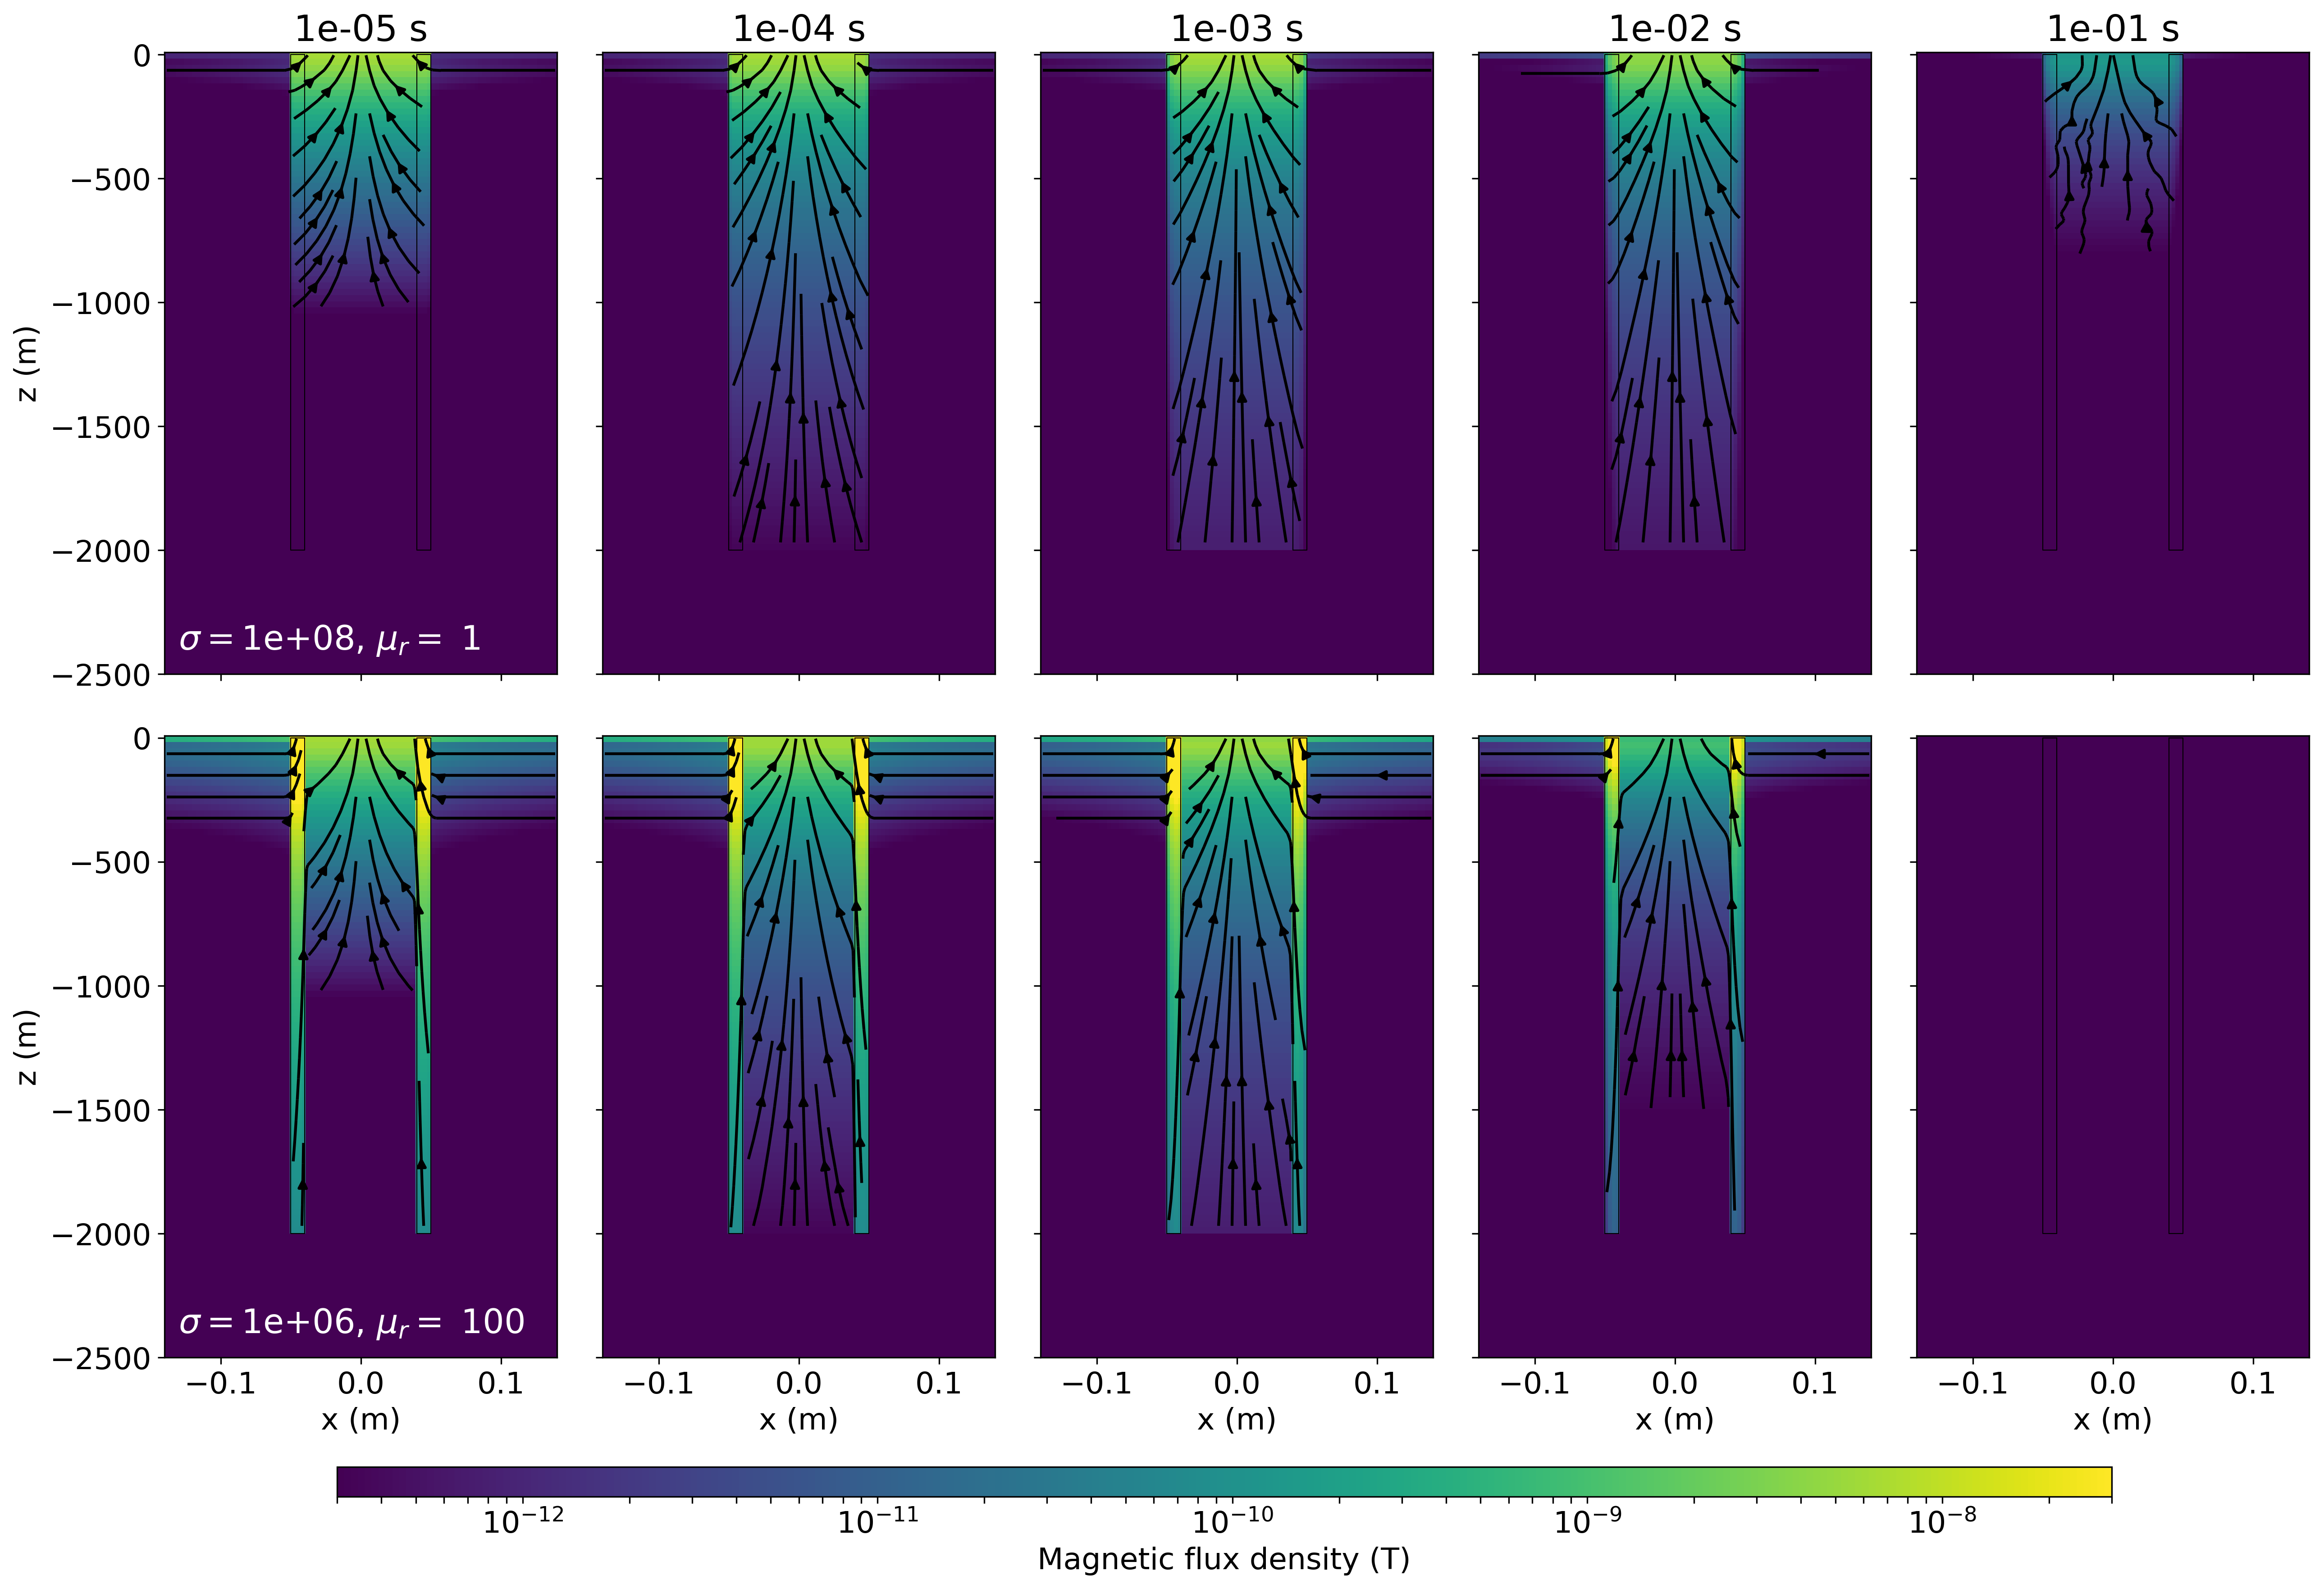
\includegraphics[width=\columnwidth]{figures/casing_software/btdem.png}
    \end{center}
\caption{
    Secondary magnetic flux density for a conductive well (top row) and a conductive, permeable well (bottom row) through time.
    The source waveform is a step-off waveform.
}
\label{fig:btdem}
\end{figure}



It is important to note that although the product of the conductivity and permeability is identical for these wells, the geometry of the well and inducing fields results in different couplings for each of the parameters. For a vertical magnetic dipole source, the electric fields are purely rotational while the magnetic fields are primarily vertical. An approximation we can use to understand the implications of these geometric difference is to assume the inducing fields are uniform (e.g. the radius of the source loop is infinite) and to examine the conductance and permeance of the pipe. For rotational electric fields, the conductance is
\begin{equation}
    \mathcal{S} = \sigma \frac{t L}{2 \pi r}
    \label{eq:conductance}
\end{equation}

where $t$ is the thickness of the casing, $r$ is the radius of the casing and $L$ is the length-scale of the pipe segment contributing to the signal. For vertical magnetic fields, the permeance is
\begin{equation}
    \mathcal{P} = \mu \frac{ t 2 \pi r}{L}
    \label{eq:permeance}
\end{equation}

As the length-scale, $L$, is larger than the circumference of the pipe ($2\pi r$) the geometric contribution to the conductance is larger than that to the permeance.

An important take-away from this example is that the contributions of conductivity and permeability to the observed EM signals are not simply governed by their product. The geometry of the source fields plays an important role in how each contributes. Thus to accurately model conductive, permeable pipes, over a range of frequencies or times, a numerical code must allow both variable conductivity and variable permeability to be considered.





\section{Summary and Outlook}

We have introduced a finite volume approach for solving Maxwell’s equations on 2D and 3D cylindrical meshes. The medium can have variable electrical conductivity and magnetic permeability. The 2D solution is especially computationally efficient and has a large number of practical applications. When cylindrical symmetry is not valid, the 3D solution can be implemented; a judicious design of the mesh can often generate a problem with fewer cells than would be required with a tensor or OcTree mesh. We demonstrated the versatility of the codes by modelling the electromagnetic fields that result when a highly conductive and permeable casing is embedded in the earth. This application was chosen because it is of current interest in the geophysical community and because the large contrasts in physical properties and length scales make it a numerically challenging problem.

We presented a number of different experiments involving DC, frequency domain, and time domain sources. Our numerical examples emulated experiments that have previously been published; this allowed us not only to verify statements made in those papers, but also to build upon them by further investigating the EM phenomena. Of critical importance was the ability to plot the charges, fields, and fluxes in the simulations. This is valuable for understanding the responses obtained from the experiment and it is a solid foundation for designing a field survey. Although our numerical results were in accordance with those in the published literature, we found some results that are not generally talked about or possibly known. For instance, in the DC problem, when a current electrode is attached to the well-head, there is an unexpected increase in charge density very close to the end of the well. For a conductive and permeable casing, excited by a circular current source, there is a complicated magnetic field that occurs in the top few centimeters of the pipe. Both of these phenomena might be due to the complexities of fields that result when a change in geometry causes a discontinuity in the definition of the normal component of the surface. Although we do not have a solid mathematical expression to explain these results, the important point to be made here is that ability to simulate fine scale structure and plot the resultant charges and fields enabled us to interrogate these phenomena.


The software implementation is included as a part of the SimPEG ecosystem. SimPEG also includes finite volume simulations on 3D tensor and OcTree meshes as well as machinery for solving inverse problems. This means that the cylindrical codes can be readily connected to an inversion and additionally, simulations and inversions of more complex 3D geologic settings can be achieved by coupling the cylindrical simulation with a 3D tensor or OcTree mesh using a primary-secondary approach (e.g. example 3 in \cite{Heagy2017}). Beyond modelling steel cased wells, we envision that the 3D cylindrical mesh could prove to be useful in conducting 3D airborne EM inversions where a domain-decomposition approach, similar to that described in \cite{Yang2014}, is adopted.

SimPEG and all of the further developments described in this paper are open source and freely available; all of the examples can be accessed at https://github.com/simpeg-research/heagy\_2018\_emcyl. The examples have been provided as Jupyter notebooks. This not only allows all of the figures in the paper to be reproduced, but provides an avenue by which the reader can ask questions, change parameters, and use resultant images to confirm (or not) his or her presumed outcome. We hope that our efforts to make the software and examples accessible promotes the utility of this work for the wider community.


